% ----------------------------------------------------------------------------
% File: analyse.tex
% Usage:        Latex2e
% Creation :  19-1-2011 morvan@enib.fr
% Revised:    
% Revised:   
% ----------------------------------------------------------------------------
\documentclass[12pt, a4paper]{book}
% ----------------------------------------------------------------------------
%-------------------------------------------------------------------------
\usepackage{helvet}
%\usepackage{psboxit,pstcol}

\usepackage[francais]{babel}
\usepackage[latin1]{inputenc}
\usepackage{moreverb}
%\usepackage{eurosym}
\usepackage{index}
\usepackage{amsfonts}
\usepackage{graphics}
\usepackage{listings}
\usepackage{hyperref}
%\usepackage{html}
\usepackage{multimedia}
\usepackage{pgfpages}
\usepackage{pgf,xcolor,tikz}
\usepackage{rotating}
\usepackage{framed}
\usepackage[framed,hyperref,standard]{ntheorem}
\usepackage{fancyhdr,lastpage}

%-------------------------------------------------------------------------
% --- Commandes --------------------------------------------------------------
\renewcommand{\chaptermark}[1]{\markboth{#1}{}}

\renewcommand\contentsname{Table des mati\`eres}
\def\ladate{mai 2015}
\def\mot-cle#1{
	{\noindent {\bf Mots-cl\'es} : #1\vspace{-.5em}\vspace{0pt}}
	\def\mot-cle{\par}
}

\def\biblio#1{\subsection{R\'ef\'erences}\list
	{[\arabic{enumi}]}{\settowidth\labelwidth{[#1]}\leftmargin\labelwidth
		\advance\leftmargin\labelsep
		\usecounter{enumi}}
	\def\newblock{\hskip .11em plus .33em minus .07em}
	\sloppy\clubpenalty4000\widowpenalty4000
	\sfcode`\.=1000\relax}
\let\endbiblio=\endlist


% --- Identification du document ---------------------------------------------
\def\soustitre{\bf\sc Logiciel d'aide � la navigation maritime en 3D}
\def\projet{\bf\sc NaVisu}
\def\sousprojet{\bf\sc Manuel utilisateur}
\def\titre{\bf\sc NaVisu }
\def\auteur{\sc{Lithops}}
\def\leclient{Projet Open Source}
\def\lauteur{Lithops}
\def\leverif{l}
\def\chef{Lithops}
\def\lechef{sm}
\def\laversion{1.0}
\def\sujet{\sc Manuel utilisateur} 

% --- Mise en page ------------------------------------------------------------
\setlength{\textwidth}{17.5cm}
\setlength{\textheight}{24.6cm}
\headsep=2cm
\footskip=1.5cm
\hoffset=-2cm
\voffset=-2.5cm
%--------------------------------------------------------------------------
% Changement de la syntaxe de la commande \chapter

\makeatletter 
\begin{comment}
\renewcommand{\@makechapterhead}[1]{
\parindent \z@ \raggedright \reset@font
\hbox to \hsize{%
\rlap{\raisebox{-2.7em}{\raisebox{\depth}{%

\includegraphics[width=9.5em]{images/logonavisuglobenoir.png}}}}%
\rlap{\hbox to 9.5em{\hss
\reset@font\sffamily\fontsize{8em}{8em}\selectfont\white 
\thechapter\hss}}%
\hspace{10em}%
\vbox{%
\advance\hsize by -10em
\reset@font\sffamily\bfseries\Huge
#1
\par
}%
}%
\vskip 20pt
\hrulefill
\vskip 50pt
} 
\def\@makeschapterhead#1{%
\parindent \z@ \raggedright \reset@font
\hbox to \hsize{%
\rlap{\raisebox{-2.7em}{\raisebox{\depth}{%

\includegraphics[width=9.5em]{images/logonavisuglobenoir.png}}}}%
\hspace{10em}%
\vbox{%
\advance\hsize by -10em
\reset@font\sffamily\bfseries\Huge
#1
\par
}%
}%
\vskip 20pt
\hrulefill
\vskip 50pt
}
\makeatother
\end{comment}
%-------------------------------------------------------------------------
\hypersetup{
	bookmarks=true,         % show bookmarks bar?
	unicode=false,          % non-Latin characters in Acrobat�s bookmarks
	pdftoolbar=true,        % show Acrobat�s toolbar?
	pdfmenubar=true,        % show Acrobat�s menu?
	pdffitwindow=false,     % window fit to page when opened
	pdfstartview={FitH},    % fits the width of the page to the window
	pdftitle={My title},    % title
	pdfauthor={Lithops},     % author
	pdfsubject={NaVisu},   % subject of the document
	pdfcreator={Lithops},   % creator of the document
	pdfproducer={Producer}, % producer of the document
	pdfkeywords={keyword1} {key2} {key3}, % list of keywords
	pdfnewwindow=true,      % links in new window
	colorlinks=false,       % false: boxed links; true: colored links
	linkcolor=red,          % color of internal links
	citecolor=green,        % color of links to bibliography
	filecolor=magenta,      % color of file links
	urlcolor=cyan           % color of external links
}

%--------------------------------------------------------------------------
\pgfdeclareimage[width=2cm,interpolate=true]{navisuLogo}{images/logonavisuglobe}

\pagestyle{fancy}
\fancyhead[LE,LO]{\pgfuseimage{navisuLogo}}
\fancyhead[CE,CO]{\sc Logiciel d'aide � la navigation maritime en 3D }
\fancyhead[RE,RO]{2015 -- \thepage/\pageref{LastPage}}
\fancyfoot[LE,LO]{}
\fancyfoot[CE,CO]{\pgfuseimage{footline-enib-adresse}}
\fancyfoot[RE,RO]{}
\renewcommand{\headrulewidth}{0pt}
\renewcommand{\footrulewidth}{0pt}

\addto\captionsfrenchb{\renewcommand\chaptername{}}

%--------------------------------------------------------------------------
\cfoot{
\includegraphics[width=18.5cm]{images/bas-page-masterPPT_RVB_final.png}}
\rfoot{\raisebox{.3cm}{\textcolor{black}{\scriptsize{Version \laversion \ - 
				\ladate}}}}

%\SetWatermarkText{\sc Projet}
%\SetWatermarkScale{4}
\begin{document}
	
% --- Commandes --------------------------------------------------------------
\newcommand{\nav}{{\sc NaVisu}}
\newcommand{\ccc}{C$^{3}$}

% ----------------------------------------------------------------------------
\begin{titlepage}
% ---------------
\begin{center}
{\LARGE\sc Association Terre Virtuelle}\\
\vspace{2cm}
\mbox{\LARGE \sc Projet NaVisu}\\
\vspace{1cm}
\href{https://github.com/terre-virtuelle/navisu.git}{https://github.com/terre-virtuelle/navisu.git}\\
\vspace{2cm}
\mbox{\LARGE \sc Dossier de d�veloppement}\\
\vspace{1cm}

\begin{bfseries}

\begin{Huge}
\soustitre
\end{Huge}

\vspace{.8cm}

\null\vfill

%%%%%%%%%%%%%%%%%%%%%%%%%%%%%%%%%%%%%%%%%%%%%%%%%%%%%%%%%%%%%%%%%%%%%%

\begin{center}
	 \href{https://github.com/terre-virtuelle/navisu.git}{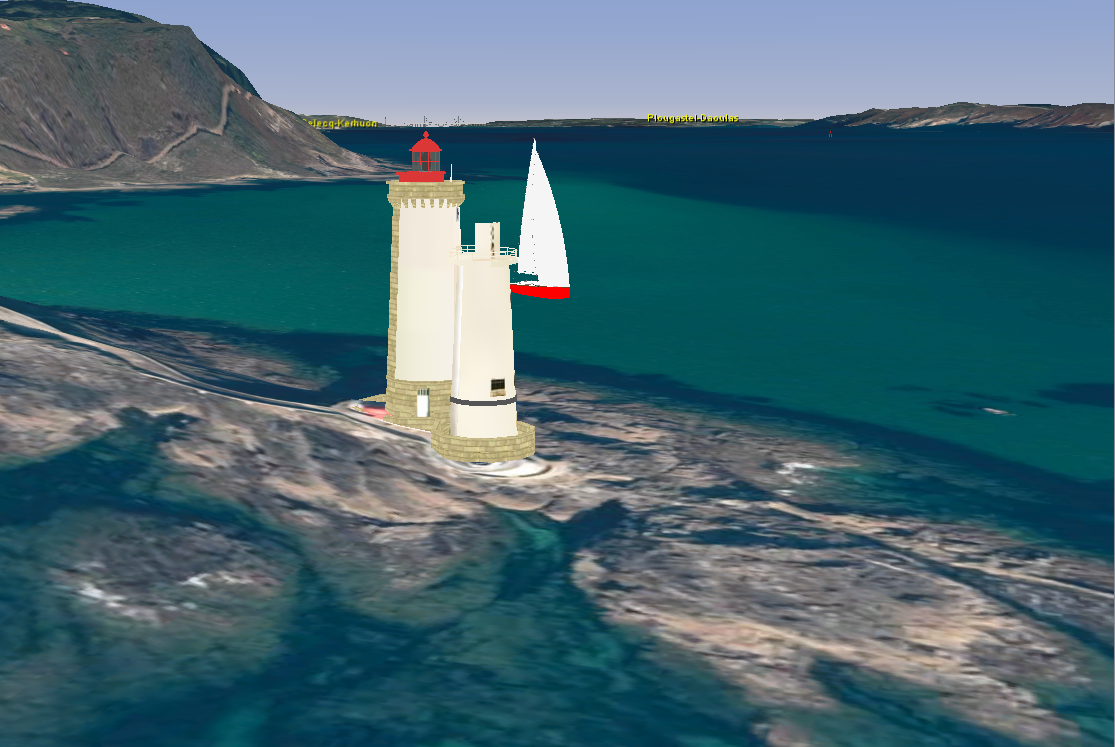
\includegraphics[width=16cm]{images/leMinou.png}}
\end{center}

%%%%%%%%%%%%%%%%%%%%%%%%%%%%%%%%%%%%%%%%%%%%%%%%%%%%%%%%%%%%%%%%%%%%%%%
\null\vfill

\vspace{1cm}
2016

\end{bfseries}
\end{center}

\end{titlepage}

\hbox{}
\newpage
% -------------------

% --- Tracabilite du document
\section*{Tra\c cabilit\'e du document}
\section*{R\'edaction}


\section*{Personnes ayant particip\'ees au projet}

\begin{tabular}{|l|} \hline
Noms \\
\hline
3dphi \\
jojal29 \\
lithops \\
mhyrdin \\
tibus29 \\
\hline
\end{tabular}



\section*{Historique des \'evolutions}

\begin{tabular}{|l|l|} \hline
Version         & Date        \\ 
\hline 
   1.0         &   mai 2015  \\
\hline 
   1.1         &   \ladate   \\
\hline
\end{tabular}

\vfill
\vspace{1cm}{\em Image de couverture : Entr�e du goulet de Brest, le phare du
petit Minou (France)}

\newpage
\hbox{}
\newpage


% --- Table des matieres ---
\tableofcontents

\hbox{}
\newpage

% --- Table des figures ---
\listoffigures

\newpage
\hbox{}
\newpage
\chapter{Architecture et fonctionnalit�s du serveur de donn�es}


\section{Pr�sentation}
Le module d'acquisition de donn�es de \nav\  est distribu�. Un serveur re�oit les donn�es des diff�rents capteurs
les analyse, les traite puis les distribue au format XML [ou JSON (option)] aux diff�rents clients. Dans la version la plus compacte serveur et client se trouvent sur une m�me machine.
 Le protocole de communication utilis� sont les WebSockets. \footnote{\href{http://fr.wikipedia.org/wiki/WebSocket}{http://fr.wikipedia.org/wiki/WebSocket}} ce protocole permet les actions bidirectionnelles, {\em push} et {\em pull}, avec les clients. Actuellement seules les requ�tes {\em pull} venant des clients sont prises en compte, mais il est simple d'introduire des actions {\em push} de la part du serveur pour des remont�es d'alarmes par exemple.
 Le protocole WebSocket est impl�ment� dans la plupart des langages actuellement.
 L'impl�mentation du serveur repose sur le {\em framework } Vert.x \footnote{\href{http://vertx.io/}{http://vertx.io/}}
 \footnote{\href{http://fr.wikipedia.org/wiki/Vert.x}{http://fr.wikipedia.org/wiki/Vert.x}}, ce {\em framework} assure la communication asynchrone entre les entr�es et les sorties du serveur, � l'aide de bus �v�nementiels : {\tt EventBus}.
 Il est simple � utiliser, ne n�cessite pas d'installation particuli�re. 
 L'int�r�t de la distribution est la possibilit� des d�velopper des clients ayant 
 diff�rentes technologies d'interfaces : JavaFX, HTML5 et diff�rents OS : Windows7/Windows8, Mac OS, iOS, Linux ou Android. les clients peuvent �tre une application \nav\ compl�te ou de simple affichages de donn�es capteurs : des instruments par exemple, ou des clients de communication type chat.
 
 %%%%%%%%%%%%%%%%%%%%%%%%%%%%%%%%%%%%%%%%%%%%%%%%%%%%%%%%%%%%%%%%%%%%%%%
 \begin{center}
 \framebox[1\width]{
 	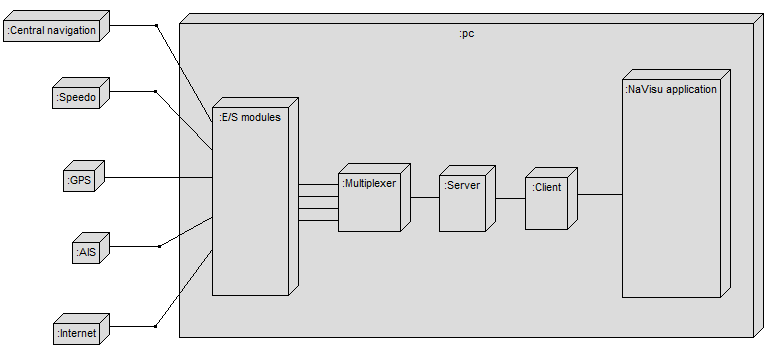
\includegraphics[width=16cm,height=10cm]{images/dataserver/deploiement_0.png}
 }
 \begin{figure}[ht]
 \caption{\label{3}\textit{D�ploiement centralis�}}
 \end{figure}
 \end{center}
 %%%%%%%%%%%%%%%%%%%%%%%%%%%%%%%%%%%%%%%%%%%%%%%%%%%%%%%%%%%%%%%%%%%%%%%
 \begin{center}
 \framebox[1\width]{
 	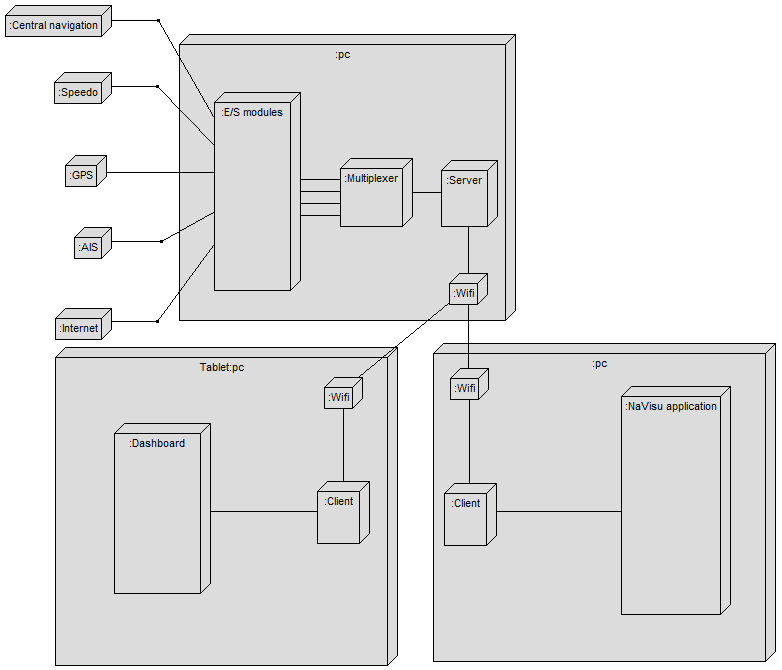
\includegraphics[width=16cm,height=10cm]{images/dataserver/deploiement_1.png}
 }
 \begin{figure}[ht]
 \caption{\label{3}\textit{D�ploiement distribu�}}
 \end{figure}
 \end{center}

 \section{Les donn�es en entr�e}
 Les donn�es sont envoy�es au serveur via les ports s�rie, USB ou Internet.
 Il est aussi possible d'avoir des donn�es � partir de fichiers, pour un rejeu de parcours par exemple.
 L'acquisition de donn�es est r�alis�e par des objets {\bf\tt Reader}, 
 \begin{center}
   \begin{minipage}{16cm}
   \begin{itemize}
   \item {\bf\tt SerialReader} pour la communication s�rie
   \item {\bf\tt HTTPReader} pour la saisie sur internet
   \item {\bf\tt FileReader} pour la lecture de donn�es sur disque
   \end{itemize}
   \end{minipage}
 \end{center}  
  Le composant {\bf\tt DataServer} peut cr�er en dynamique les diff�rents {\bf\tt Reader} et les param�trer.
  Exemples de  d�bits sur les ports s�rie : 
  \begin{center}
  \begin{minipage}{16cm}
  \begin{itemize}
  \item 4800 bauds (GPS, centrale de navigation, \ldots, NMEA0183 ASCII)
  \item 38400 bauds (AIS, NMEA0183 binaire)
  \item 250 Kbits/sec (GPS, centrale de navigation, moteurs, \ldots,N2K binaire)
  \end{itemize}
  \end{minipage}
  \end{center} 
   Exemples de  frames pour les entr�es capteurs :
    {\small
    \begin{verbatim}
 NMEA0183  : $GPRMC,093518.470,A,4826.2552,N,00429.8708,W,000.0,203.5,051113,,,A*7A
 AIS       : !AIVDM,1,1,,B,13IMVT0000OcEt8KcIfW75F@0<0>,0*52
 NMEA 2000 : <0x18eeff01> [8] 05 a0 be 1c 00 a0 a0 c0
    \end{verbatim}
    }
\section{L'architecture}\footnote{Dans les figures qui suivent les flux de donn�es dynamiques sont colori�s en turquoise, les canaux de communication en gris clair.}

%%%%%%%%%%%%%%%%%%%%%%%%%%%%%%%%%%%%%%%%%%%%%%%%%%%%%%%%%%%%%%%%%%%%%%%
\begin{center}
\framebox[1\width]{
	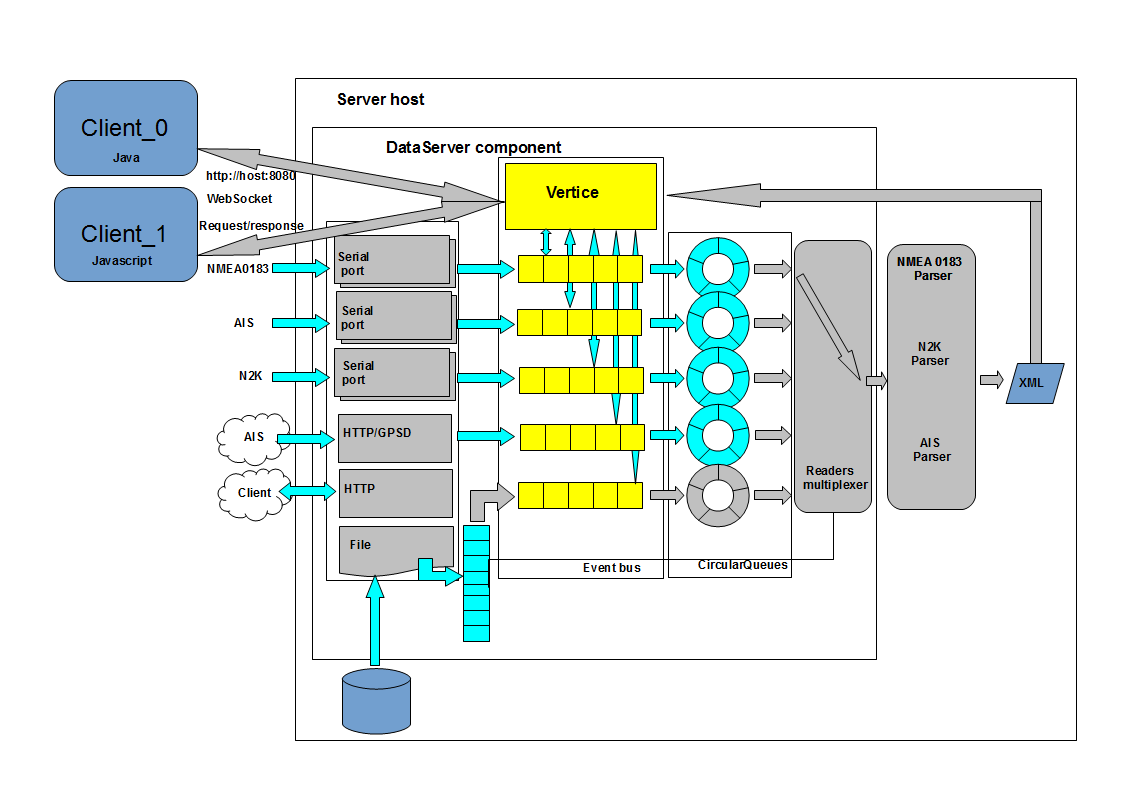
\includegraphics[width=16cm,height=12cm]{images/dataserver/dataServer_0.png}
	}
\begin{figure}[ht]	
\caption{\label{1}\textit{Aucune requ�te client, les donn�es dynamiques venant des capteurs sont perdues}}
\end{figure}
\end{center}
%%%%%%%%%%%%%%%%%%%%%%%%%%%%%%%%%%%%%%%%%%%%%%%%%%%%%%%%%%%%%%%%%%%%%%%
Un {\bf\tt Reader} sp�cialis� est associ� � chaque entr�e, un bus d'�v�nements Vert.x lui est attribu�, ainsi
qu'une file circulaire.
En entr�e continu les donn�es sont envoy�es, via leur bus, � leur file. En sortie le d�bit d'acquisition  est pilot� par chaque client.Si il n'y a pas de requ�tes client, les
nouvelles donn�es �crasent les anciennes, sauf pour celles venant de fichiers qui sont transf�r�es int�gralement.
Un s�lecteur de {\bf\tt Reader} assure le multiplexage des donn�es, actuellement la strat�gie du choix est simple parcours circulaire, mais une strat�gie avec file � priorit� peut �tre facilement mise en \oe uvre. Sur requ�te d'un client
la file circulaire active d�livre ses donn�es au s�lecteur d'analyseur syntaxique: NMEA0183, AIS, N2K. 
Le parseur choisi traite les donn�es, g�n�re des objets NMEA, les transforme au format XML et les envoie � l'objet {\bf\tt Vertice} qui les envoie au client. Une nouvelle file est s�lectionn�e dans l'attente d'une autre requ�te client.
Les donn�es sont donc analys�es ({\em pars�es}) deux fois, une premi�re fois par le parseur NMEA sp�cialis�, une deuxi�me fois par le client � partir de d'un format XML. Ceci se justifie par le fait que l'�criture du premier parseur est complexe du fait de la grande variabilit� des formats NMEA, les connexions �lectriques avec les capteurs peuvent aussi engendrer  
un bruitage des donn�es, ces donn�es sont ensuite mises en forme suivant un sch�ma XML unique, les clients n'ont aucune difficult�s � les transformer en objets � partir de l'API JAXB. D�s que le format JSON sera bien int�gr� � JEE, ce
format sera pr�f�r� � XML. D'autres protocoles, tel que CoAP sont envisageables dans l'avenir.
\section{La dynamique}
%%%%%%%%%%%%%%%%%%%%%%%%%%%%%%%%%%%%%%%%%%%%%%%%%%%%%%%%%%%%%%%%%%%%%%%
\begin{center}
\framebox[1\width]{
	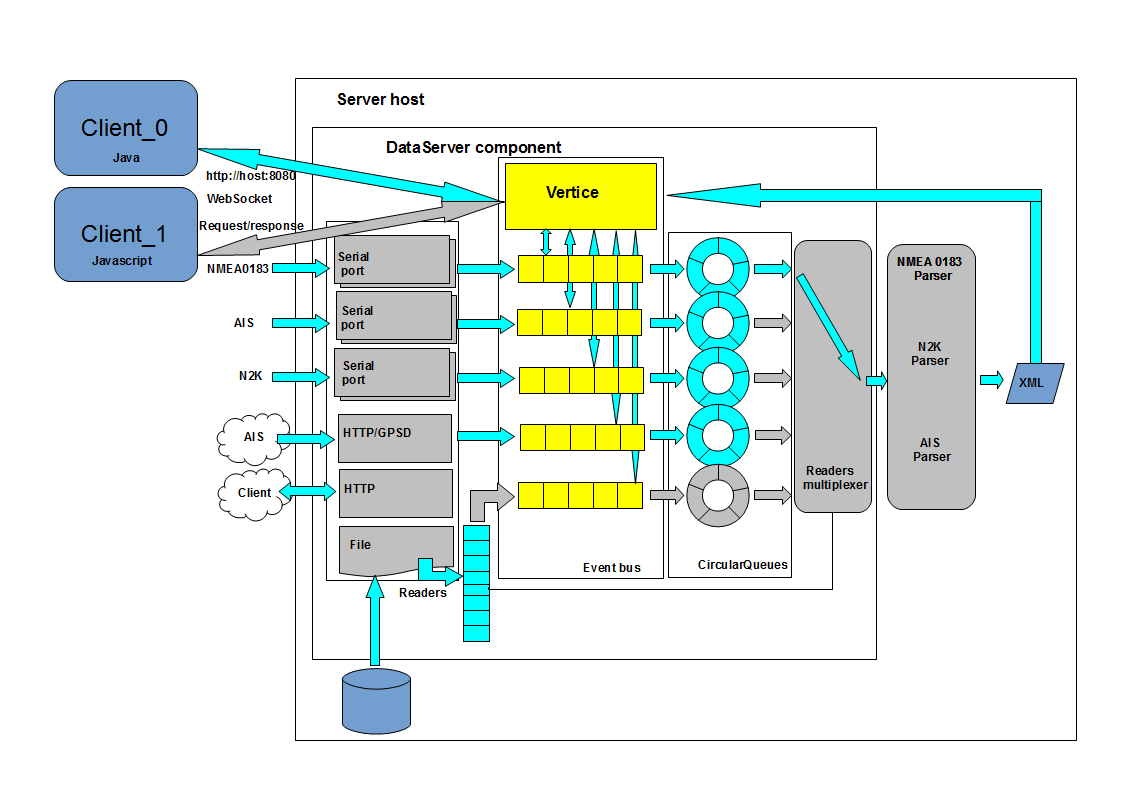
\includegraphics[width=16cm,height=12cm]{images/dataserver/dataServer_1.png}
}
\begin{figure}[ht]
\caption{\label{2}\textit{Exemple de requ�te client, suivie d'une r�ponse asynchrone � partir du premier port s�rie enregistr�.}}
\end{figure}
\end{center}

\subsection{Performances}
En test, le serveur supporte une requ�te client toutes les milisecondes, dans la pratique, un navire naviguant � 15 n\oe uds 
parcourt 7.5m en une seconde, un barreur va r�gler le d�bit d'affichage des donn�es � 2 ou 3 secondes. Une p�riode de 
1 seconde pour les requ�tes semble raisonnable.
%%%%%%%%%%%%%%%%%%%%%%%%%%%%%%%%%%%%%%%%%%%%%%%%%%%%%%%%%%%%%%%%%%%%%%%
\begin{center}
\framebox[1\width]{
	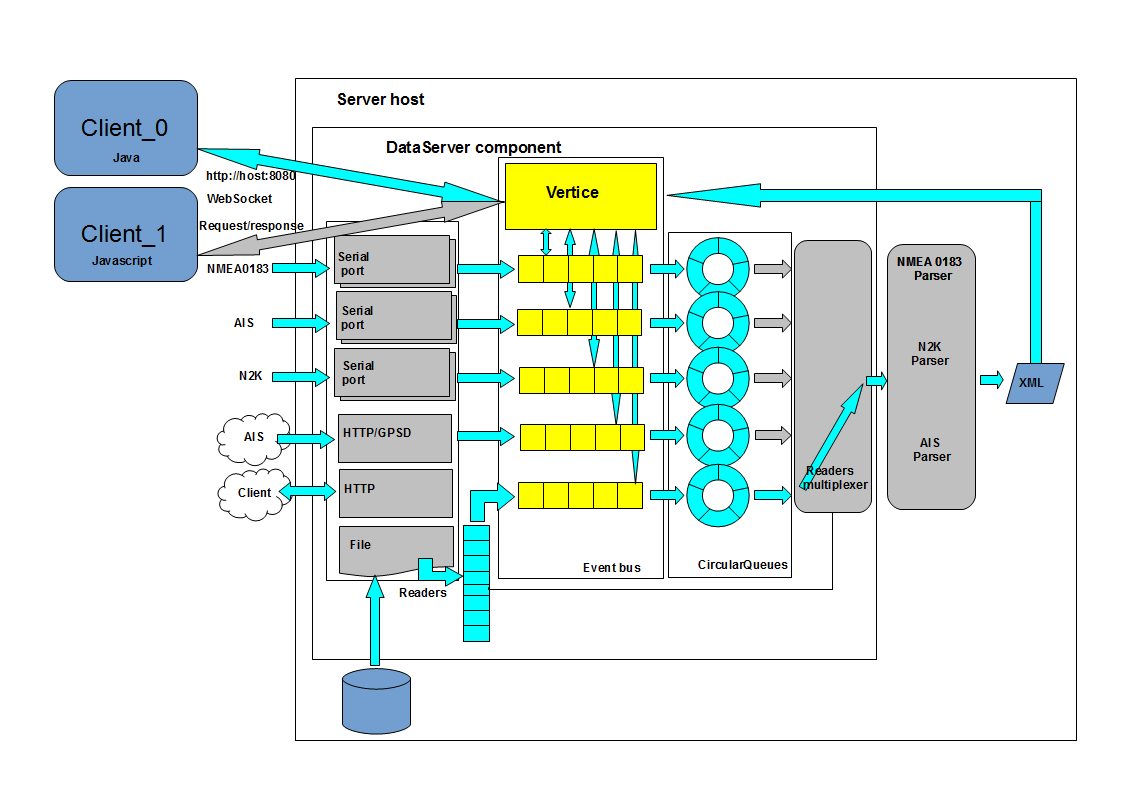
\includegraphics[width=16cm,height=12cm]{images/dataserver/dataServer_2.png}
}
\begin{figure}[ht]
\caption{\label{3}\textit{Exemple de requ�te client, suivie d'une r�ponse synchrone � partir de donn�es provenant d'un fichier.}}
\end{figure}
\end{center}
%%%%%%%%%%%%%%%%%%%%%%%%%%%%%%%%%%%%%%%%%%%%%%%%%%%%%%%%%%%%%%%%%%%%%%%
\section{Les donn�es en sortie (extrait)}
{\small
 \begin{verbatim}
<?xml version="1.0" encoding="UTF-8" standalone="true"?>
-<sentences>
-<rmc>
  <device>GP</device>
  <sentence>
    $GPRMC,191137.304,A,4826.2620,N,00429.8665,W,000.0,225.3,050114,,,A*7C
  </sentence>
  <eastOrWestVariation/>
  <date>2014-01-05T19:11:37.972+01:00</date>
  <status>A</status>
  <latitude>48.437702</latitude>
  <longitude>-4.4977746</longitude>
  <variation>0.0</variation>
  <track>225.3</track>
  <sog>0.0</sog>
</rmc>
-<gga>
  <device>GP</device>
  <sentence>
    $GPGGA,191138.000,4826.2632,N,00429.8614,W,2,05,1.2,72.4,M,52.1,M,0.8,0000*50
  </sentence>
  <utc>2014-01-05T19:11:38.973+01:00</utc>
  <latitude>48.43772</latitude>
  <longitude>-4.4976897</longitude>
  <gpsQualityIndicator>2</gpsQualityIndicator>
  <numberOfSatellitesInView>5</numberOfSatellitesInView>
  <horizontalDilutionOfPrecision>1.2</horizontalDilutionOfPrecision>
  <antennaAltitude>72.4</antennaAltitude>
  <unitsOfAntennaAltitude>M</unitsOfAntennaAltitude>
  <geoidAltitude>52.1</geoidAltitude>
  <unitsOfGeoidAltitude>M</unitsOfGeoidAltitude>
  </gga>
</sentences>
\end{verbatim}
}

\chapter{Installation et personnalisation du serveur de donn�es \nav}

%Ref : TV050714\_TU\_SM \hfill R�dacteur : Serge  Morvan \\

\section{Pr�sentation}
    Ce tutoriel fait suite � celui ci : Architecture et fonctionnalit�s du serveur de donn�es . Il a pour objet l'explication de la d�marche compl�te d'installation, de param�trisation, voire de la modification, du serveur de donn�es capteurs. Ce serveur fait l'acquisition  des donn�es, assure leur multiplexage ainsi que la diffusion de ces donn�es au format {\tt xml}. Il est n�cessaire d'installer ce serveur, dans le cas d'une application distribu�e o� l'acquisition et la visualisation ne se fait pas compl�tement ou uniquement au sein de NaVisu.

 \begin{center}
 \framebox[1\width]{
 	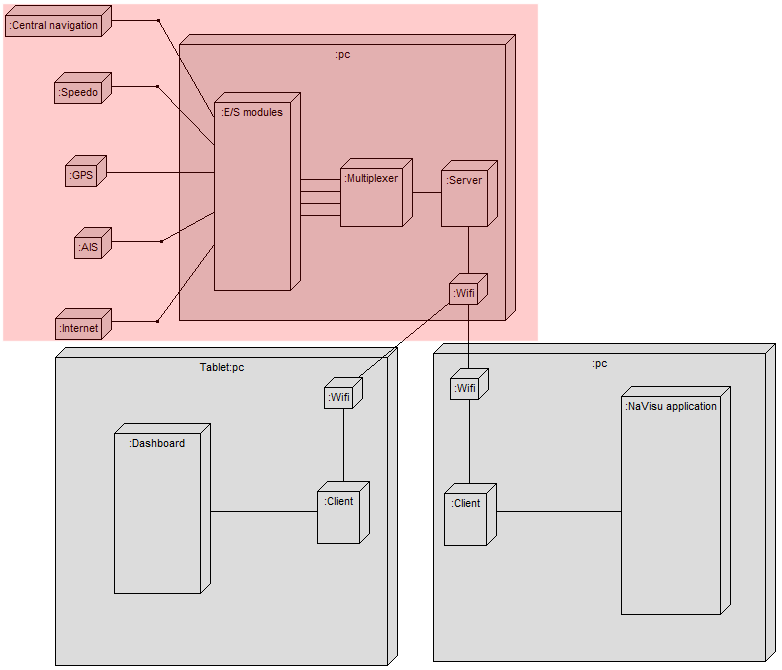
\includegraphics[width=16cm,height=10cm]{images/server/deploiement_2.png}
 }
 \begin{figure}[ht]
 \caption{\label{3}\textit{D�ploiement distribu�}}
 \end{figure}
 \end{center}

 \section{Le projet}
   Le projet \nav\  est divis� en sous-projets, chaque sous-projet poss�de une architecture type composants.
 La plupart des  sous-projets sont d�velopp�s sous forme d'API, ayant le minimun de d�pendance avec les autres sous-projets.
 C'est le cas de l'API {\tt navisu-server}, qui ne d�pend que du module {\tt navisu-domain} : description des mod�les d'objets utilis�s. Il est donc simple de pr�senter le serveur sous forme d'un projet ind�pendant.
\section{T�l�chargement}
\href{https://github.com/terre-virtuelle/Navisu-server.git}{https://github.com/terre-virtuelle/Navisu-server.git}
\section{Param�trisation}
l'API NaVisu-server ne fourni pas d'IHM, pour la param�trisation, celle ci se fait � l'aide du fichier de propri�t�s : {\tt properties/server.properties} 
\begin{verbatim}
#  NmeaServer properties file

#File name for tests without serial comm
fileName = data/nmea/gps.txt

# Web server parameters
hostName = localhost
port = 8080
queueSize = 5

# Serial parameters
# [portNumber - 1] for Linux
portNumber = 5
# COM for Windows OS, /dev/ttyS for Linux
portName = COM5
baudRate = 4800
dataBits = 8
stopBits = 1
parity = 0
\end{verbatim}

Modifier les param�tres en fonction de votre configuration. Attention � la d�nomination diff�rente des ports sous Windows et sous Linux.\\
La variable {\tt port} correspondant au num�ro du port de communication avec les clients, attention de n'avoir pas d�j� des applications utilisant ce port.

\section{Lancement}
 A partir du fichier jar : {\tt java -jar NaVisuServer.jar}
 
 \newpage 
 \section{D�veloppement}
 
 La classe de test est : {\tt bzh.terrevirtuelle.navisu.server.app.ServerMain }\\
 

 \begin{verbatim}
        ComponentManager componentManager = ComponentManager.componentManager; 
         // deploy components
         LOGGER.log(Level.INFO, "\n Start", componentManager.startApplication(
                 DataServerImpl.class
         ));
         DataServerServices nmeaServerServices = 
                  componentManager.getComponentService(DataServerServices.class);
        
         // Test avec choix des parametres de comm
         // nmeaServerServices.init("localhost", 8080);
         // nmeaServerServices.openSerialPort("COM4", 4800, 8, 1, 0);
         // nmeaServerServices.openSerialPort("COM5", 4800, 8, 1, 0);
         
         
         // Test avec les parametres de comm dans properties/nmea.properties
         nmeaServerServices.init();
         nmeaServerServices.openSerialPort(); 
         // nmeaServerServices.openFile();     
\end{verbatim}

La premi�re partie du code est relative � la gestion des composants. Ensuite deux s�ries d'exemples
la premi�re s�rie fixe dans le code les param�tres d'acquisition et de diffusion. La deuxi�me s�rie
utilise les valeurs par d�faut indiqu�es dans le fichier de propri�t�s. L'initialisation doit �tre 
unique, par contre on peut ouvrir autant d'entr�es que l'on veut.
\chapter{Les donn�es NMEA 0183}

%Ref : TV080114\_TU\_SM \hfill R�dacteur : Serge  Morvan \\



\section{Le standard NMEA}
http://standards.nmea.org/
Le site officiel : \\
 \hbox{}\hspace{1cm}\href{http://www.nmea.org/}{http://www.nmea.org/} \\
 Des informations sur le contenu des phrases : \\
 \hbox{}\hspace{1cm}\href{http://gpsinformation.net/}{http://gpsinformation.net/}\\
 \hbox{}\hspace{1cm}\href{http://gpsd.berlios.de/NMEA.html}{http://gpsd.berlios.de/NMEA.html}\\
 \hbox{}\hspace{1cm}\href{http://www.kh-gps.de/nmea.faq}{http://www.kh-gps.de/nmea.faq}\\
 Un projet de service d�mon :\\
 \hbox{}\hspace{1cm}\href{http://catb.org/gpsd/}{http://catb.org/gpsd/}\\

\newpage
\section{Mod�le NMEA0183}
\subsection{Ensemble des phrases analys�es}
\begin{center}
\framebox[1\width]{
	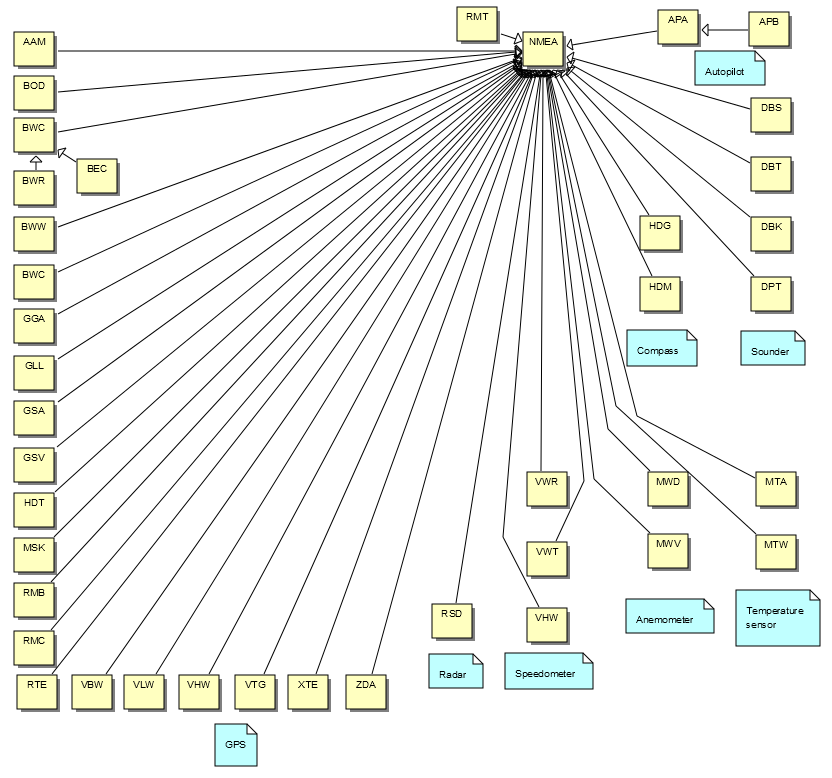
\includegraphics[width=18cm]{images/nmea/nmea.png}
}
\begin{figure}[h]
\caption{\label{nmea}\textit{Ensemble des classes de l'API NMEA}}
\end{figure}
\end{center}
%%%%%%%%%%%%%%%%%%%%%%%%%%%%%%%%%%%%%%%%%%%%%%%%%%%%%%%%%%%%%%%%%%%%%%%
%%%%%%%%%%%%%%%%%%%%%%%%%%%%%%%%%%%%%%%%%%%%%%%%%%%%%%%%%%%%%%%%%%%%%%
\begin{center}
\framebox[1\width]{
	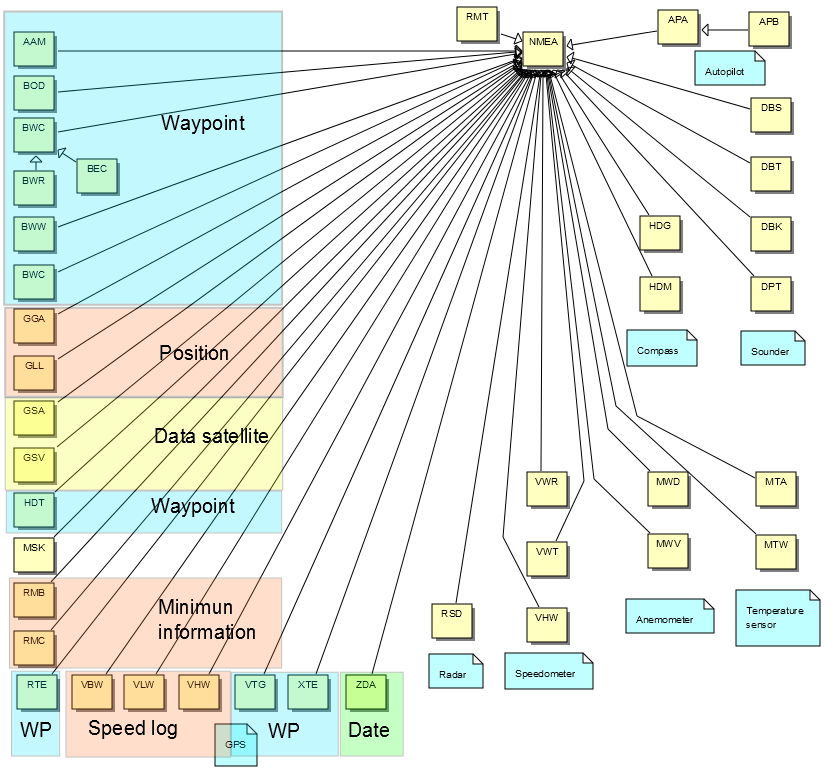
\includegraphics[width=17cm]{images/nmea/nmea_comment.png}
}
\begin{figure}[h]
\caption{\label{repart}\textit{Cat�gorisation des informations NMEA}}
\end{figure}
\end{center}
%%%%%%%%%%%%%%%%%%%%%%%%%%%%%%%%%%%%%%%%%%%%%%%%%%%%%%%%%%%%%%%%%%%%%%%
%%%%%%%%%%%%%%%%%%%%%%%%%%%%%%%%%%%%%%%%%%%%%%%%%%%%%%%%%%%%%%%%%%%%%%
\subsection{Minimun d'information pour la navigation}
\begin{center}
\framebox[1\width]{
	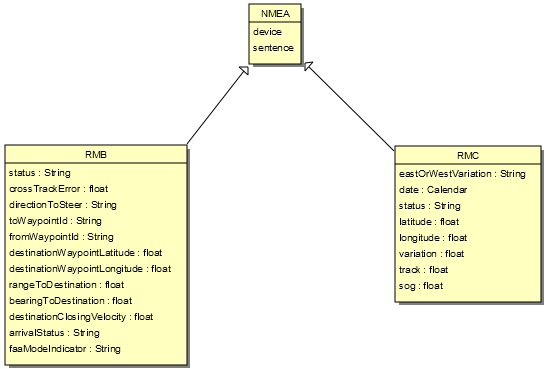
\includegraphics[width=16cm]{images/nmea/gps_minimum.png}
}
\begin{figure}[h]
\caption{\label{gpsminimum}\textit{Minimun d'information pour la navigation}}
\end{figure}
\end{center}
%%%%%%%%%%%%%%%%%%%%%%%%%%%%%%%%%%%%%%%%%%%%%%%%%%%%%%%%%%%%%%%%%%%%%%%
%%%%%%%%%%%%%%%%%%%%%%%%%%%%%%%%%%%%%%%%%%%%%%%%%%%%%%%%%%%%%%%%%%%%%%
\subsection{Date et heure}
\begin{center}
\framebox[1\width]{
	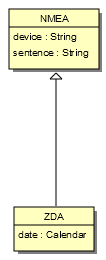
\includegraphics[width=3cm]{images/nmea/date.png}
}
\begin{figure}[h]
\caption{\label{date}\textit{Date}}
\end{figure}
\end{center}
%%%%%%%%%%%%%%%%%%%%%%%%%%%%%%%%%%%%%%%%%%%%%%%%%%%%%%%%%%%%%%%%%%%%%%%
%%%%%%%%%%%%%%%%%%%%%%%%%%%%%%%%%%%%%%%%%%%%%%%%%%%%%%%%%%%%%%%%%%%%%%
\subsection{Position : latitude, longitude}
\begin{center}
\framebox[1\width]{
	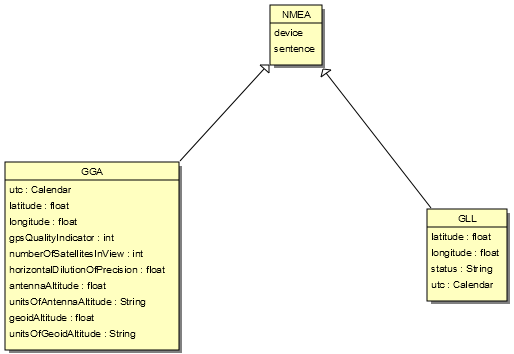
\includegraphics[width=16cm]{images/nmea/position.png}
}
\begin{figure}[h]
\caption{\label{position}\textit{Informations de position}}
\end{figure}
\end{center}
%%%%%%%%%%%%%%%%%%%%%%%%%%%%%%%%%%%%%%%%%%%%%%%%%%%%%%%%%%%%%%%%%%%%%%%
%%%%%%%%%%%%%%%%%%%%%%%%%%%%%%%%%%%%%%%%%%%%%%%%%%%%%%%%%%%%%%%%%%%%%%
\subsection{Informations de vitesse et de distance}
\begin{center}
\framebox[1\width]{
	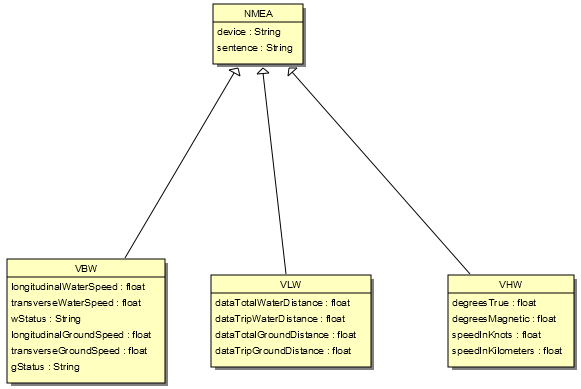
\includegraphics[width=16cm]{images/nmea/speedLog.png}
}
\begin{figure}[h]
\caption{\label{speedLog}\textit{Informations de vitesse et de distance}}
\end{figure}
\end{center}
%%%%%%%%%%%%%%%%%%%%%%%%%%%%%%%%%%%%%%%%%%%%%%%%%%%%%%%%%%%%%%%%%%%%%%%
%%%%%%%%%%%%%%%%%%%%%%%%%%%%%%%%%%%%%%%%%%%%%%%%%%%%%%%%%%%%%%%%%%%%%%
\subsection{Informations sur les waypoints}
\begin{center}
\framebox[1\width]{
	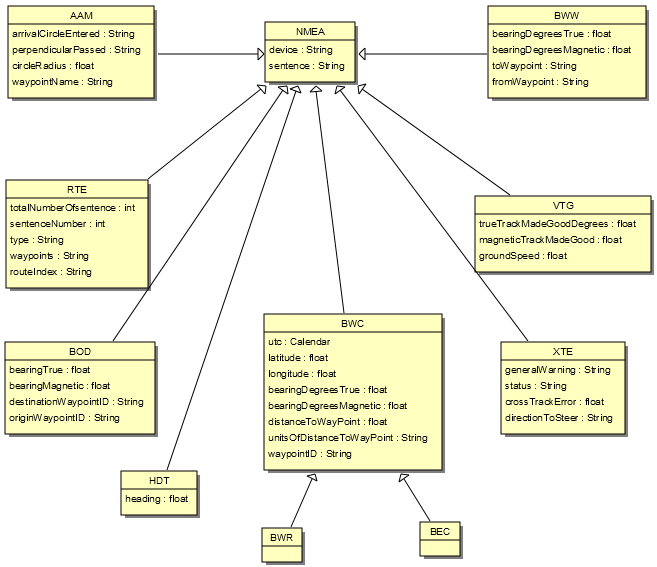
\includegraphics[width=16cm]{images/nmea/waypoint.png}
}
\begin{figure}[h]
\caption{\label{waypoint}\textit{Informations sur les waypoints}}
\end{figure}
\end{center}
%%%%%%%%%%%%%%%%%%%%%%%%%%%%%%%%%%%%%%%%%%%%%%%%%%%%%%%%%%%%%%%%%%%%%%%
%%%%%%%%%%%%%%%%%%%%%%%%%%%%%%%%%%%%%%%%%%%%%%%%%%%%%%%%%%%%%%%%%%%%%%
\subsection{Informations sur les satellites}
\begin{center}
\framebox[1\width]{
	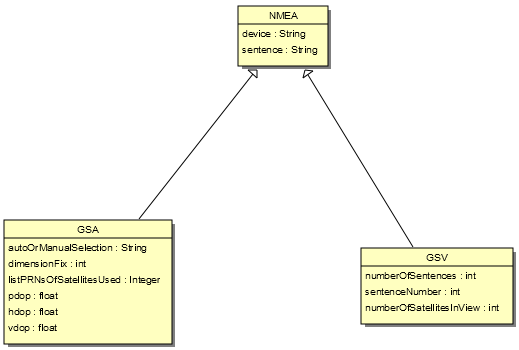
\includegraphics[width=16cm]{images/nmea/satellite.png}
}
\begin{figure}[h]
\caption{\label{satellite}\textit{Informations sur les satellites}}
\end{figure}
\end{center}

%%%%%%%%%%%%%%%%%%%%%%%%%%%%%%%%%%%%%%%%%%%%%%%%%%%%%%%%%%%%%%%%%%%%%%%
%%%%%%%%%%%%%%%%%%%%%%%%%%%%%%%%%%%%%%%%%%%%%%%%%%%%%%%%%%%%%%%%%%%%%%
\subsection{Informations sur le vent}
\begin{center}
\framebox[1\width]{
	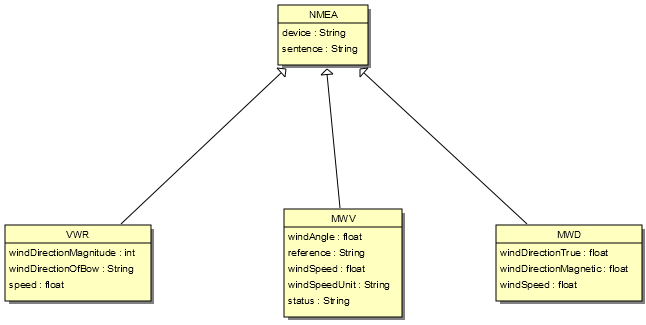
\includegraphics[width=16cm]{images/nmea/anemometer.png}
}
\begin{figure}[h]
\caption{\label{anemometer}\textit{Informations sur le vent}}
\end{figure}
\end{center}
%%%%%%%%%%%%%%%%%%%%%%%%%%%%%%%%%%%%%%%%%%%%%%%%%%%%%%%%%%%%%%%%%%%%%%%
%%%%%%%%%%%%%%%%%%%%%%%%%%%%%%%%%%%%%%%%%%%%%%%%%%%%%%%%%%%%%%%%%%%%%%
\subsection{Bathym�trie}
\begin{center}
\framebox[1\width]{
	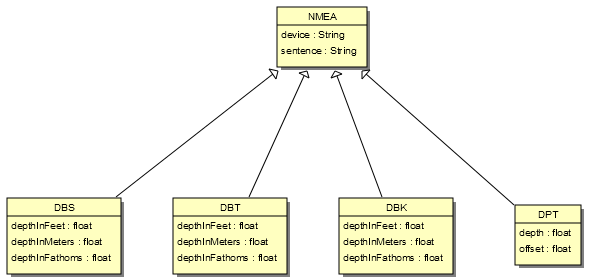
\includegraphics[width=16cm]{images/nmea/depth.png}
}
\begin{figure}[h]
\caption{\label{depth}\textit{Bathym�trie}}
\end{figure}
\end{center}
%%%%%%%%%%%%%%%%%%%%%%%%%%%%%%%%%%%%%%%%%%%%%%%%%%%%%%%%%%%%%%%%%%%%%%%

 %%%%%%%%%%%%%%%%%%%%%%%%%%%%%%%%%%%%%%%%%%%%%%%%%%%%%%%%%%%%%%%%%%%%%%
 \section{Pr�sentation de l'API}
 L'API permet l'acc�s au mod�le NMEA que nous avons choisit, celui-ci est proche
 de l'ensemble des phrases mais s'en �loigne parfois lorsqu'il y a redondance
 d'information dans une phrase, plusieurs valeurs de vitesse dans diff�rentes
 unit�s par exemple, ou lorsqu'une structure plus �labor�e permet de stocker des
 donn�es : liste, dictionnaire, \ldots
 \subsection{L'analyseur lexical et syntaxique}
 Le standard NMEA a beaucoup �volu�, plusieurs constructeurs ont impos� leur
 modifications, ce qui fait que de nombreuses variantes apparaissent dans les
 sorties NMEA des diff�rents appareils. Nous avons choisi d'uiliser le g�n�rateur
 d'analyseurs lexicaux et syntaxiques ANTLR pour plus de clart� du code. \\
 \hbox{}\hspace{1cm}\href{http://www.antlr.org/}{http://www.antlr.org/} \\
 \newpage
 En plus de cet outil nous utilisons l'atelier ANTLRWorks : \\ 
 \hbox{}\hspace{1cm}\href{http://www.antlr.org/works/}{http://www.antlr.org/works/}
 \\ Cet atelier permet de visualiser les grammaires cr��es.
 \subsubsection{Un exemple simple} 
 \small
 \begin{verbatim}
 GSV	     : '$' device=DEVICE 'GSV' 
 (NUMBER | SEP)+ 
 checksum=CHECKSUM
 { //action }
 \end{verbatim}
 \normalsize{}
 \begin{center}
 	\framebox[1\width]{
 		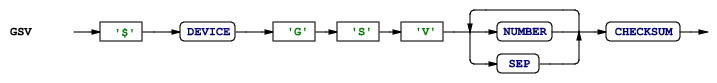
\includegraphics[width=12cm]{images/nmea/gsv.png}
 	}
 	\begin{figure}[h]
 		\caption{\label{gsv}\textit{Analyse de la phrase GSV}}
 	\end{figure}
 \end{center}
 
 \subsubsection{Un exemple plus complexe}
 \small
 \begin{verbatim}
 RMB     : '$' device = DEVICE 'RMB' SEP 
 status = LETTERS SEP  
 (crossTrackError =  NUMBER)* SEP
 (directionToSteer = LETTERS)* SEP
 (fromWaypointId = LETTERS |fromWaypointId = NUMBER)*  SEP
 (toWaypointId =  LETTERS | toWaypointId = NUMBER)* SEP
 (destinationWaypointLatitude =  NUMBER)* SEP (ns = LETTERS)* SEP
 (destinationWaypointLongitude  =  NUMBER)* SEP (ew  = LETTERS)* SEP
 (rangeToDestination =  NUMBER)* SEP
 (bearingToDestination =  NUMBER)* SEP
 (destinationClosingVelocity =  NUMBER)* SEP 	        	    
 (LETTERS SEP)*
 (arrivalStatus = LETTERS | '\u0000')* 
 checksum=CHECKSUM 
 { // action}
 \end{verbatim}
 \normalsize{}
 \begin{center}
 	\framebox[1\width]{
 		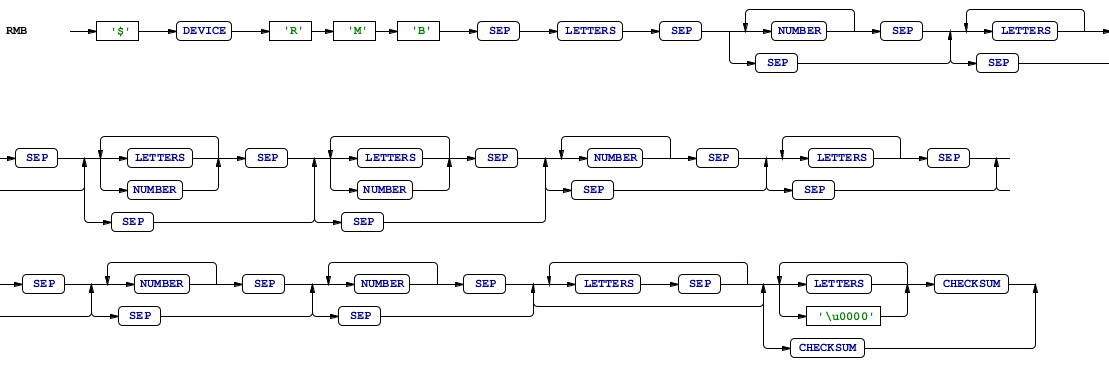
\includegraphics[width=12cm]{images/nmea/rmb.png}
 	}
 	\begin{figure}[h]
 		\caption{\label{dbt}\textit{Analyse de la phrase RMB}}
 	\end{figure}
 \end{center}
 
 %%%%%%%%%%%%%%%%%%%%%%%%%%%%%%%%%%%%%%%%%%%%%%%%%%%%%%%%%%%%%%%%%%%%%%

%%%%%%%%%%%%%%%%%%%%%%%%%%%%%%%%%%%%%%%%%%%%%%%%%%%%%%%%%%%%%%%%%%%%%%%

\section{Glossaire}
\begin{tabular}{|l|l|l|}
\hline
\bf Acronyme & \bf Expansion \\
\hline
AAM & Waypoint Arrival Alarm  \\
\hline
ALM & GPS Almanac Data \\
\hline
APA & Autopilot Sentence ``A''\\
\hline
APB  & Autopilot Sentence ``b''\\
\hline
BEC & Bearing and Distance to Waypoint,  Dead Reckoning\\
\hline
BOD & Bearing, Waypoint to Waypoint\\
\hline
BWC & Bearing and Distance to Waypoint\\
\hline
BWR  & Bearing and Distance to Waypoint   \\
\hline
BWW & Bearing and  Waypoint to Waypoint \\
\hline
DBK & Depth Below Keel \\
\hline
DBS & Depth Below Surface \\
\hline
DBT & Depth Below Transducer \\
\hline
DPT & Depth and offset \\
\hline
GGA &  Global Positioning System Fix Data. Time \\
\hline
GLL & Geographic Position and Latitude/Longitude \\
\hline
GSA & GPS DOP and active satellites \\
\hline
GSV & Satellites in view \\
\hline
GTD & Geographic Location in Time Differences \\
\hline
HDG & Heading, Deviation and Variation \\
\hline
HDM & Heading Magnetic \\
\hline
HDT & Heading True \\
\hline
MTW & Water Temperature \\
\hline
MWV & Wind Speed and Angle \\
\hline
RMA & Recommended Minimum Navigation Information \\
\hline
RMB & Recommended Minimum Navigation Information \\
\hline
RMC & Recommended Minimum Navigation Information \\
\hline
RTE & Routes \\
\hline
VBW & Dual Ground/Water Speed \\
\hline
VHW & Water Speed and Heading \\
\hline
VLW & Distance Traveled through Water \\
\hline
VPW & Speed, Measured Parallel to Wind \\
\hline
VTG & Track Made Good and Ground Speed \\
\hline
VWR & Relative Wind Speed and Angle \\
\hline
XTE & Cross-Track Error  Measured \\
\hline
ZDA & Time, Date and UTC, Day, Month, Year and Local Time Zone \\
\hline
\end{tabular}


\chapter{Architecture et fonctionnalit�s du client NMEA}

%Ref : TV240114\_TU\_SM \hfill R�dacteur : Serge  Morvan \\


\section{Les connexions au serveur}
Les diff�rents p�riph�riques et capteurs fournissent les donn�es de navigation au serveur, suivant diff�rents
protocoles. Ces donn�es sont multiplex�es par le serveur. Sur requ�te des clients elles sont analys�es, transform�es dans un format XML standard et envoy�es aux diff�rents clients. Ces clients peuvent �tre sur la m�me machine dans
le cas le plus simple ou sur d'autres ordinateurs, tablettes ou smartphones. \nav\ est le client le plus riche.
%%%%%%%%%%%%%%%%%%%%%%%%%%%%%%%%%%%%%%%%%%%%%%%%%%%%%%%%%%%%%%%%%%%%%%%
\begin{center}
\framebox[1\width]{
	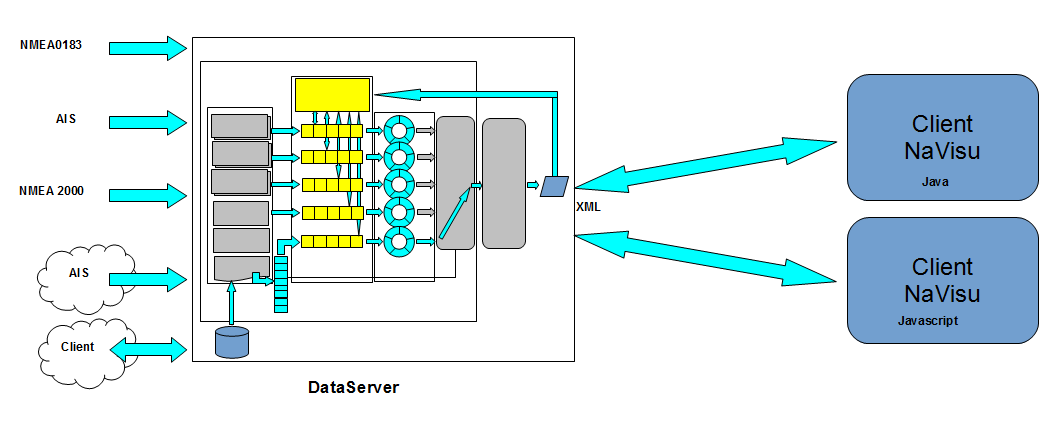
\includegraphics[width=16cm]{images/dataServer_3.png}
}
\begin{figure}[ht]
\caption{\label{0}\textit{Sch�ma g�n�ral des entr�es/sorties}}
\end{figure}
\end{center}
%%%%%%%%%%%%%%%%%%%%%%%%%%%%%%%%%%%%%%%%%%%%%%%%%%%%%%%%%%%%%%%%%%%%%%%
\section{Les donn�es en entr�e}
Il n'existe pas, � notre connaissance, de sch�ma XML bien d�fini pour l'ensemble des donn�es NMEA.
A l'exception de quelques cas particuliers comme : GPX  \footnote{\href{http://www.topografix.com/gpx.asp}{http://www.topografix.com/gpx.asp}}
ou AIS  \footnote{\href{http://www.thsoa.org/hy07/04P\?_10.pdf}{http://www.thsoa.org/hy07/04P\_10.pdf}} par exemple.
Nous avons donc d�fini notre propre mod�le NMEA \footnote{Voir article Mod�le NMEA} associ� � un sch�ma nmea.xsd structurant les donn�es
sans ambigu�t�s et permettant leur validation.
\subsection{Extrait du sch�ma {\tt nmea.xsd}}
{\small
 \begin{verbatim}
<xs:complexType name="gga">
  <xs:sequence>
    <xs:element name="device" type="xs:string" minOccurs="0"/>
    <xs:element name="sentence" type="xs:string" minOccurs="0"/>
    <xs:element name="utc" type="xs:dateTime" minOccurs="0"/>
    <xs:element name="latitude" type="xs:float"/>
    <xs:element name="longitude" type="xs:float"/>
    <xs:element name="gpsQualityIndicator" type="xs:int"/>
    <xs:element name="numberOfSatellitesInView" type="xs:int"/>
    <xs:element name="horizontalDilutionOfPrecision" type="xs:float"/>
    <xs:element name="antennaAltitude" type="xs:float"/>
    <xs:element name="unitsOfAntennaAltitude" type="xs:string" minOccurs="0"/>
    <xs:element name="geoidAltitude" type="xs:float"/>
    <xs:element name="unitsOfGeoidAltitude" type="xs:string" minOccurs="0"/>
  </xs:sequence>
</xs:complexType>
\end{verbatim}
}
\subsection{Extrait d'un fichier de donn�es conforme au sch�ma {\tt nmea.xsd}}
{\small
 \begin{verbatim}
<?xml version="1.0" encoding="UTF-8" standalone="true"?>
-<sentences>
  -<gga>
    <device>GP</device>
    <sentence>
      $GPGGA,191138.000,4826.2632,N,00429.8614,W,2,05,1.2,72.4,M,52.1,M,0.8,0000*50
    </sentence>
    <utc>2014-01-05T19:11:38.973+01:00</utc>
    <latitude>48.43772</latitude>
    <longitude>-4.4976897</longitude>
    <gpsQualityIndicator>2</gpsQualityIndicator>
    <numberOfSatellitesInView>5</numberOfSatellitesInView>
    <horizontalDilutionOfPrecision>1.2</horizontalDilutionOfPrecision>
    <antennaAltitude>72.4</antennaAltitude>
    <unitsOfAntennaAltitude>M</unitsOfAntennaAltitude>
    <geoidAltitude>52.1</geoidAltitude>
    <unitsOfGeoidAltitude>M</unitsOfGeoidAltitude>
 </gga>
</sentences>
\end{verbatim}
}
\newpage
\section{Le projet {\tt NaVisuSimpleClient}}

   Le projet \nav est divis� en sous-projets, chaque sous-projet poss�de une architecture type composants.
 La plupart des  sous-projets sont d�velopp�s sous forme d'API, ayant le minimun de d�pendance avec les autres sous-projets.
 C'est le cas de l'API {\tt navisu-client}, qui ne d�pend que du module {\tt navisu-domain} : description des mod�les d'objets utilis�s. Il est donc simple de pr�senter le serveur sous forme d'un projet ind�pendant : {\tt NaVisuSimpleClient}
 
\section{T�l�chargement}
\href{https://github.com/terre-virtuelle/NaVisu-client.git}{https://github.com/terre-virtuelle/NaVisu-client.git}
\section{Param�trisation}
l'API NaVisu-client ne fourni pas d'IHM, pour la param�trisation, celle ci se fait � l'aide du fichier de propri�t�s : {\tt properties/client.properties} 
\begin{verbatim}
# Web client parameters
hostName = localhost
port = 8080
period = 1000
\end{verbatim}

La variable {\tt port} correspondant au num�ro du port de communication avec les clients, attention de n'avoir pas d�j� des applications utilisant ce port. 

\section{Lancement}
 A partir du fichier jar : {\tt java -jar NaVisuSimpleClient.jar}

 \section{D�veloppement}
 Le serveur fourni les donn�es � l'aide du protocole WebSocket, le client doit donc se
 conformer � ce protocole. La propri�t�  period permet de modifier la fr�quence d'acquisition des donn�es sur le client. Le protocole WebSocket permet des actions en pull ou en push. Nous avons fait le choix de faire l'acquisition uniquement 
 en mode pull. Le client d�cide d'envoyer une requ�te : {\tt nmea} au serveur qui lui renvoie un paquet de donn�es. Entre deux requ�tes les donn�es arriv�es sur le serveur peuvent �tre perdues. Pour le client \nav, pr�sent� ici nous avons choisi d'utiliser le framework {\tt Vert.x }, comme pour le serveur, mais tout autre solution est possible.
 \footnote{\href{http://vertx.io/}{http://vertx.io/}}
 
 
 \hbox{}\newpage
 La classe de test est : {\tt bzh.terrevirtuelle.navisu.client.app.ClientMain }\\
 
 \begin{verbatim}
  ComponentManager componentManager = ComponentManager.componentManager;
  // deploy components
  LOGGER.log(Level.INFO, "\n Start", componentManager.startApplication(
          NmeaClientImpl.class
  ));
  NmeaClientServices nmeaClientServices = 
         componentManager.getComponentService(NmeaClientServices.class);
           
 nmeaClientServices.open("localhost", 8080);
 nmeaClientServices.request(100); 
\end{verbatim}
La premi�re partie est relative aux composants, ensuite le client se connecte sur le serveur, sur le port 8080 puis fait des requ�tes
toutes les 100 millisecondes.

\section{Diffusion de donn�es}
 Dans l'exemple pr�sent�, les donn�es re�ues sont pars�es � 
l'aide de l'API JAXB \footnote{\href{https://jaxb.java.net/}{https://jaxb.java.net/}}. Nous utilisons le support
de la programmation �v�nementielle de \ccc. A chaque objet NMEA 
instanci�, l'�v�nement correspondant est �mis et diffus� aupr�s des abonn�s. 
{\small
 \begin{verbatim}
 public interface NMEAEvent
         extends ComponentEvent {
     public <T extends NMEA> void notifyNmeaMessageChanged(T data);
 }
 
 public interface GGAEvent
         extends NMEAEvent {
 } 
 \end{verbatim}
 }
\section{Ecriture d'un souscripteur � un �v�nement}
L'inscription � la r�ception d'�v�nements d'un type particulier suit la d�marche de \ccc :
  \begin{enumerate}
  \item Recherche du {\tt componentManager}
  \item Recherche de l'objet de souscription � un �v�nement particulier {\tt ggaES }
  \item Souscription et sur-d�finition de la m�thode r�ponse {\tt notifyNmeaMessageChanged(T data)}
  \item La m�thode �tant g�n�rique, l'h�ritage des �v�nements NMEA, n'�tant pas un v�ritable h�ritage, 
  il convient d'appliquer une coercition de type afin d'analyser les donn�es re�ues.
  \item Traitement des donn�es.
  \end{enumerate}
  
  \subsection{Exemple de souscription et de traitement apr�s r�ception d'un �v�nement type {\tt GGA}}
  {\small
 \begin{verbatim}
public class Locator {

    ComponentManager cm = ComponentManager.componentManager;
    ComponentEventSubscribe<GGAEvent> ggaES = 
                cm.getComponentEventSubscribe(GGAEvent.class);

    public Locator() {
        ggaES.subscribe(new GGAEvent() {

            @Override
            public <T extends NMEA> void notifyNmeaMessageChanged(T data) {
                GGA gga = (GGA) data;
                System.out.println("Latitude : " + gga.getLatitude()
                              + "   Longitude : " + gga.getLongitude());
            }
        });
    }
}
\end{verbatim}
}

\section{Autre d�veloppement possible}
L'�criture d'un client n'impose que le respect du protocole WebSocket, il est donc tout � fait possible d'�crire des clients dans un autre langage que java et avec une philosophie de diffusion que la programmation �v�nementielle.
Un exemple de client �l�mentaire �crit en Javascript :
\begin{verbatim}
<html>
<head><title>Web Socket Test</title></head>
<body>
<script>
    var socket;
    if (window.WebSocket) {
        socket = new WebSocket("ws://localhost:8080/nmea");
        socket.onmessage = function(event) {
            alert("Received data from websocket: " + event.data);
        }
        socket.onopen = function(event) {
            alert("Web Socket opened!");
        };
        socket.onclose = function(event) {
            alert("Web Socket closed.");
        };
    } else {
        alert("Your browser does not support Websockets. (Use Chrome)");
    }
\end{verbatim}
\newpage
\begin{verbatim}
    function send(message) {
        if (!window.WebSocket) {
            return;
        }
        if (socket.readyState == WebSocket.OPEN) {
             socket.send(message);
        } else {
            alert("The socket is not open.");
        }
    }
</script>
<form onsubmit="return false;">
    <input type="text" name="message" value="Nmea"/>
    <input type="button" value="Send Web Socket Data" 
                onclick="send(this.form.message.value)"/>
</form>
</body>
</html>
\end{verbatim}
%%%%%%%%%%%%%%%%%%%%%%%%%%%%%%%%%%%%%%%%%%%%%%%%%%%%%%%%%%%%%%%%%%%%%%%
\begin{center}
\framebox[1\width]{
	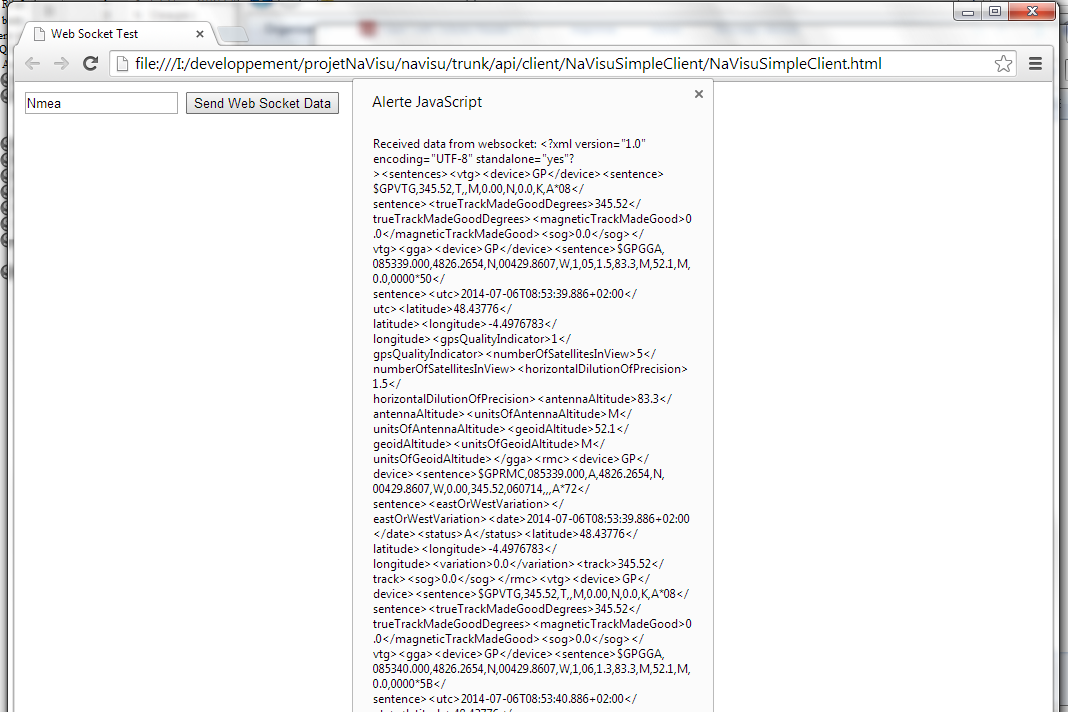
\includegraphics[width=16cm]{images/jsClient.png}
}
\begin{figure}[ht]
\caption{\label{0}\textit{Un client �l�mentaire en javascript}}
\end{figure}
\end{center}
%%%%%%%%%%%%%%%%%%%%%%%%%%%%%%%%%%%%%%%%%%%%%%%%%%%%%%%%%%%%%%%%%%%%%%%
\chapter{Cr�ation d'un nouveau Display}

Ref : TV310315\_TU\_SM \hfill R�dacteur : Serge  Morvan \\


\section{Architecture}
\subsection{Principes}
Un {\tt Display} est un composant, au sens de C$^3$, il peut ainsi b�n�ficier des services du 
composant {\tt GuiAgent} par exemple. L'application n'a aucun lien cod� avec lui. Le design du nouveau compo\-sant 
est compl�tement s�par� du code.
Chaque �l�ment variable poss�de un id. Le contr�leur, instanci� par le {\tt Display} lors de l'initialisation
charge le fichier {\tt .fxml}. On retrouve dans le code du contr�leur les id de la partie graphique.
Pr�conisations : le composant graphique principal est un {\tt Group}, son id est : {\tt view}, chaque {\tt Display}
poss�de un bouton de fermeture, dont l'id est {\tt quit}. Le contr�leur h�rite de la classe {\tt Widget2D} qui offre 
les services de l'interactivit�.
 L'attribut {\tt KEY\_NAME}, ici : {\tt "InstrumentTemplate"} permet au Dock de le rechercher et de l'afficher, lorsque l'item
 associ� est s�lectionn�. Comme ci dessous dans la classe {\tt DockManagerImpl} du module {\tt navisu-app}, lors de
 la cr�ation du Dock :
 {\small 
\begin{verbatim}
instrumentsRadialMenu = RadialMenuBuilder.create()
.centralImage("instrumentsradialmenu150.png")
.createNode(0, "navigation.png",1,"ais.png",1,"template.png",(e)->open("InstrumentTemplate"))
.build();
\end{verbatim}
}
Le nouveau {\tt Display} devra s'enregistrer aupr�s du {\tt IntrumentDriverManagerServices}, dans la classe {\tt AppMain} du module {\tt navisu-launcher}.
{\small
\begin{verbatim}
 // deploy components
 LOGGER.info("\n"
 + componentManager.startApplication(DpAgentImpl.class,
 .....
  InstrumentTemplateImpl.class
  )
  );
  ......
  InstrumentTemplateServices instrumentTemplateServices 
                   = componentManager.getComponentService(InstrumentTemplateServices.class); 
  ......
  instrumentDriverManagerServices.registerNewDriver(instrumentTemplateServices.getDriver());
\end{verbatim}
}
\subsection{Diagramme UML}
La figure ci dessous pr�sente un diagramme simplifi� pour un {\tt Display} appel� {\tt InstrumentTemplate},
%%%%%%%%%%%%%%%%%%%%%%%%%%%%%%%%%%%%%%%%%%%%%%%%%%%%%%%%%%%%%%%%%%%%%%%
\begin{center}
	\framebox[1\width]{
		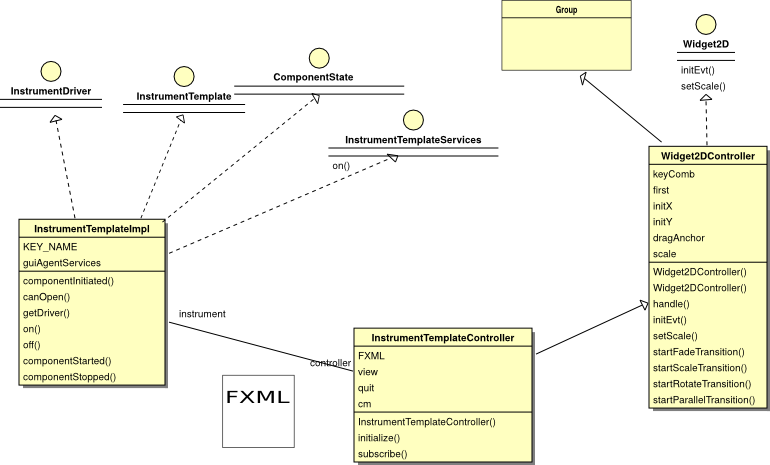
\includegraphics[width=16cm]{images/display/InstrumentTemplate.png}
	}
	\begin{figure}[ht]
		\caption{\label{0}\textit{Diagramme UML simplifi� d'un Display}}
	\end{figure}
\end{center}
%%%%%%%%%%%%%%%%%%%%%%%%%%%%%%%%%%%%%%%%%%%%%%%%%%%%%%%%%%%%%%%%%%%%%%%
\section{Cr�er un nouveau {\tt Display} : {\tt Compass}}
Reprendre le code du {\tt InstrumentTemplate}, �crire les interfaces {\tt Compass} et {\tt CompassServices}, impl�menter
les classes {\tt CompassImpl} et {\tt CompassControler}.Cr�er le fichier graphique {\tt compass.fxml}. Identifier par un id chaque variable.
Reprendre ces variables en mode public dans le contr�leur. Eventuellement ajouter des services, par d�faut
un {\tt Display} offre le service {\tt on()}. Impl�menter les contr�les.

\chapter{Cr�ation des menus}

Ref : TV110415\_TU\_SM \hfill R�dacteur : Serge  Morvan \\


\section{Objet}
Le but de cette section est d'expliquer la fa�on de rajouter un menu et ses sous-menus au Dock.
Un certain nombre de services doivent �tre activ�s, ou d�sactiv�s par l'utilisateur, pour cela, le menu
du Dock est privil�gi�. Le service � activer devra faire partie du groupe des {\tt Driver}: 
\hbox{}\vspace{0.2cm}

\begin{itemize}
 \item { \tt Driver } : pour l'ouverture de fichiers
 \item { \tt DDriver } : pour le parcours de r�pertoires   
 \item { \tt InstrumentDriver } : pour le choix d'un instrument   
 \item { \tt DatabaseDriver } : pour la connexion  � une base de donn�es
 \item { \tt WebDriver } : pour la connexion � un site web via un URL
 \item  \ldots autres � venir
\end{itemize}
Ce service doit �tre enregistr� dans le module {\tt navisu-launcher} :

\hbox{}\vspace{0.2cm}
{\small
\begin{boxedverbatim}
	
InstrumentDriverManagerServices instrumentDriverManagerServices =
         componentManager.getComponentService(InstrumentDriverManagerServices.class);
instrumentDriverManagerServices.init();
instrumentDriverManagerServices.registerNewDriver(sonarServices.getDriver());
instrumentDriverManagerServices.registerNewDriver(radarServices.getDriver());

\end{boxedverbatim}
}
\vspace{0.2cm}


Ensuite {\color{red}deux modules} sont concern�s, le module {\tt navisu-app} pour sp�cifier le nouvel item dans le Dock (ic�nes et code) et le module {\tt navisu-widgets} (ic�nes) car les {\tt RadialMenu} sont des widgets. Dans les deux cas les images sont plac�es dans les ressources, correspondant � l'arborescence des classes {\tt DockManagerImpl} et {\tt RadialMenu} respectivement. Dans la suite nous prendrons l'exemple de l'instanciation, du d�marrage ou de l'arr�t d'un {\tt Instrument}. Bien entendu cet {\tt Instrument} doit �tre impl�ment� au pr�alable.
\hbox{}\vspace{0.2cm}

{\small
	\begin{boxedverbatim}
		
public class SonarImpl
                  implements Sonar, SonarServices, InstrumentDriver, ComponentState {
	
\end{boxedverbatim}
}
\vspace{0.2cm}

\section{Le graphisme}
\subsection{Module \tt navisu-app}
	Dessiner l'ic�ne de l'item : � placer dans : \\
	{\tt bzh/terrevirtuelle/navisu/app/guiagent/dock/impl/dock\_icons} des ressources
	%%%%%%%%%%%%%%%%%%%%%%%%%%%%%%%%%%%%%%%%%%%%%%%%%%%%%%%%%%%%%%%%%%%%%%%
	\begin{center}
		\framebox[1\width]{
			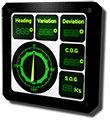
\includegraphics[width=4cm]{images/instruments.png}
		}
		\begin{figure}[ht]
			\caption{\label{0}\textit{L'item Instruments}}
		\end{figure}
	\end{center}

	%%%%%%%%%%%%%%%%%%%%%%%%%%%%%%%%%%%%%%%%%%%%%%%%%%%%%%%%%%%%%%%%%%%%%%%
	\subsection{Module \tt navisu-widgets}
	%%%%%%%%%%%%%%%%%%%%%%%%%%%%%%%%%%%%%%%%%%%%%%%%%%%%%%%%%%%%%%%%%%%%%%%
	Dessiner les ic�nes de l'item central du {\tt RadialMenu} et de ses sous-items : � placer dans : \\
	{\tt bzh.terrevirtuelle.navisu.widgets.radialmenu.menu} des ressources.
	\begin{center}
		\framebox[1\width]{
			
\includegraphics[width=4cm]{images/instrumentsradialmenu.png}
		}
			\framebox[1\width]{
				
\includegraphics[width=2cm]{images/navigation.png}
			}
			\framebox[1\width]{
				
\includegraphics[width=2cm]{images/ais.png}
			}
			\framebox[1\width]{
				
\includegraphics[width=2cm]{images/aisradar.png}
			}
			\framebox[1\width]{
				
\includegraphics[width=2cm]{images/bathy.png}
			}
		\begin{figure}[ht]
			\caption{\label{0}\textit{L'ic�ne centrale de Instruments et les sous-items}}
		\end{figure}
	\end{center}
	%%%%%%%%%%%%%%%%%%%%%%%%%%%%%%%%%%%%%%%%%%%%%%%%%%%%%%%%%%%%%%%%%%%%%%%

\section{Le code}	
\subsection{Module \tt navisu-app}
 Dans la classe {\tt DockManagerImpl} du module {\tt navisu-app}, ajouter un item au Dock  :
\hbox{}\vspace{0.2cm}

{\small
	\begin{boxedverbatim}
		
public final DockItem[] ICONS = new DockItem[]{
	DockItemFactory.newImageItem("instruments", 
	     ICON_PATH + "dock_icons/instruments.png",
    	(e) -> {
        	instrumentsRadialMenu.setVisible(!instrumentsRadialMenu.isVisible());
    	}),
    	...
    	
\end{boxedverbatim}
}

\hbox{}\vspace{0.2cm}
		Ici {\tt "instruments"} correspond � l'infobulle associ�e, {\tt ICON\_PATH+"dock\_icons/instruments.png"} 
		est le chemin de l'image dans le r�pertoire {\tt resources}. Le dernier argument du constructeur est le
		callback associ�, g�n�ralement celui l�.
Appeler la m�thode de cr�ation du {\tt RadialMenu} associ� :

\hbox{}\vspace{0.2cm}
{\small
	\begin{boxedverbatim}
		
@Override
public void makeDock() {
    createDockWidget(scene);
    createBooksRadialWidget();
    createChartsRadialWidget();
		
    createInstrumentsRadialWidget();
	
    createMeteoRadialWidget();
    createTidesRadialWidget();
    createToolsRadialWidget();
    createNavigationRadialWidget();
}

\end{boxedverbatim}
}

\hbox{}\vspace{0.2cm}
Coder cette m�thode : le menu radial est cr�� � l'aide d'un {\tt RadialMenuBuilder}

\hbox{}\vspace{0.2cm}
{\small
	\begin{boxedverbatim}
		
	//--------------INSTRUMENTS------------------
private void createInstrumentsRadialWidget() {
    instrumentsRadialMenu = RadialMenuBuilder.create()
    .centralImage("instrumentsradialmenu.png")
    .createNode(0, "navigation.png", 0, "ais.png", 0, "aisradar.png", 
		                                                (e) -> open("AisRadar"))
    .createNode(0, "navigation.png", 1, "bathy.png", 0, "sonarOn.png",
		                                                (e) -> open("Sonar"))
    .build();
		
    instrumentsRadialMenu.setLayoutX((width / 2) - 40);
    instrumentsRadialMenu.setLayoutY(height / 2);
    root.getChildren().add(instrumentsRadialMenu);
	
    radialMenus.add(instrumentsRadialMenu);
	}
	
\end{boxedverbatim}
}

\hbox{}\vspace{0.2cm}
\begin{itemize}
	\item La m�thode {\tt createNode} va pr�ciser pour chaque item, son placement, ses images associ�es et son callback.
	\begin{itemize}
		\item Un choix d'ergonomie a �t� fait, les menus radiaux ont deux couches de sous-menus puis des feuilles, les feuilles correspondent aux actions.
		\item Dans la premi�re couche les segments sont num�rot�s : 0, 1, 2, ... Dans l'exemple un seul segment,
		son ic�ne est {\tt navigation.png"}
		\item Dans la deuxi�me couche, idem, les segments sont num�rot�s : 0, 1, 2, ...Dans l'exemple deux
		segments, les ic�nes {\tt ais.png} et {\tt bathy.png}
		\item Chaque segment re�oit les feuilles correspondant aux items, ici un item par segment. 
		les images {\tt aisradar.png} et {\tt sonarOn.png} respectivement.
		\item Enfin, le dernier argument correspond au callback associ� � cet item.
	\end{itemize}
\end{itemize}

	%%%%%%%%%%%%%%%%%%%%%%%%%%%%%%%%%%%%%%%%%%%%%%%%%%%%%%%%%%%%%%%%%%%%%%%
	\begin{center}
		\framebox[1\width]{
			
\includegraphics[width=16cm]{images/menu.png}
		}
		\begin{figure}[ht]
			\caption{\label{0}\textit{Le menu Instruments}}
		\end{figure}
	\end{center}
	
	%%%%%%%%%%%%%%%%%%%%%%%%%%%%%%%%%%%%%%%%%%%%%%%%%%%%%%%%%%%%%%%%%%%%%%%	
 	\subsection{Choix des {\tt callbacks}}	
 	La plupart du temps les callbacks associ�s aux items n'ont pas besoin d'�tre cod�s, il sont fournis par \nav
 	. Ci apr�s la liste non exhaustive des calbacks et des cas d'utilisation.
 	\begin{itemize}
\item Cas d'un instrument : l'argument correspond au nom de l'instrument � activer.

	\hbox{}\vspace{0.2cm}
	{\small
		\begin{boxedverbatim}
		
private void open(String keyName) {
    instrumentDriverManagerServices.open(keyName);
    clear();
}

\end{boxedverbatim}
}

\newpage 
\item Cas d'ouverture d'un fichier : le premier argument est le {\tt KEY\_NAME} du {\tt Driver} sachant interpr�ter ces fichiers : Sedimentology, Currents, \ldots Le deuxi�me argument le ou les extensions des fichiers : {\tt .shp, .SHP} ou {\tt .000} par exemple.

\hbox{}\vspace{0.2cm}
	{\small
		\begin{boxedverbatim}
			
private void open(String description, String... des) {
    String[] tab = new String[des.length];	
    int i = 0;
    for (String s : des) {
        tab[i] = "*" + s;
        i++;
    }
    driverManagerServices.open(description, tab);
    clear();
}

\end{boxedverbatim}
}

\hbox{}\vspace{0.2cm}
\item Connexion � une base de donn�es :

\hbox{}\vspace{0.2cm}
{\small
	\begin{boxedverbatim}
		
private void openDB(String dbName, String hostName, String protocol, String port,
String driverName, String userName, String passwd) {
    databaseDriverManagerServices.connect(dbName, hostName, protocol, 
                                            port, driverName, userName, passwd);
    clear();
}
		
	\end{boxedverbatim}
}

	\hbox{}\vspace{0.2cm}
\nav\ g�re autant de bases de donn�es qu'il est n�cessaire, elles doivent �tre install�es au pr�alable, sauf pour une base embarqu�e. C'est l'API JDBC qui est exhib�e comme un ensemble de services.

\end{itemize}
\hbox{}\vspace{0.2cm}

	\subsection{Module  \tt navisu-widgets}
	Pas de code � �crire, il faut simplement placer les images correspondant au menu et � ses items, dans le fichier {\tt resources}.
%%%%%%%%%%%%%%%%%%%%%%%%%%%%%%%%%%%%%%%%%%%%%%%%%%%%%%%%%%%%%%%%%%%%%%%
\section{Principe des {\tt DriverManager}}
Comme il a �t� dit dans la pr�face, les services accessibles � partir du menu doivent s'enregistrer, voici l'explication. Le premier principe respect� est {\color{red} l'inversion de d�pendance} : la logique de l'application, contenue dans le module {\tt navisu-app} ne doit pas d�pendre des modules quelle active :
%%%%%%%%%%%%%%%%%%%%%%%%%%%%%%%%%%%%%%%%%%%%%%%%%%%%%%%%%%%%%%%%%%%%%%%
\begin{center}
	\framebox[1\width]{
		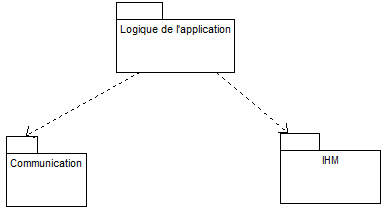
\includegraphics[width=9cm]{images/dip_0.png}
	}
	\begin{figure}[ht]
		\caption{\label{0}\textit{Une modification de l'IHM va impacter l'application}}
	\end{figure}
\end{center}
%%%%%%%%%%%%%%%%%%%%%%%%%%%%%%%%%%%%%%%%%%%%%%%%%%%%%%%%%%%%%%%%%%%%%%%	
La logique de l'application  doit s'appuyer sur des services :
%%%%%%%%%%%%%%%%%%%%%%%%%%%%%%%%%%%%%%%%%%%%%%%%%%%%%%%%%%%%%%%%%%%%%%%
\begin{center}
	\framebox[1\width]{
		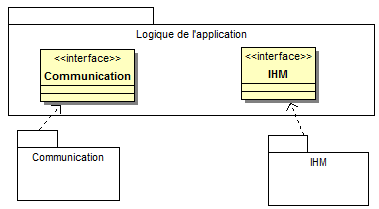
\includegraphics[width=9cm]{images/dip_1.png}
	}
	\begin{figure}[ht]
		\caption{\label{0}\textit{Si les contrats de services sont respect�s, un changement du code de l'IHM ne concerne pas l'application}}
	\end{figure}
\end{center}
%%%%%%%%%%%%%%%%%%%%%%%%%%%%%%%%%%%%%%%%%%%%%%%%%%%%%%%%%%%%%%%%%%%%%%%	
Le deuxi�me principe est celui de  {\color{red}pas de d�pendances cycliques} :
%%%%%%%%%%%%%%%%%%%%%%%%%%%%%%%%%%%%%%%%%%%%%%%%%%%%%%%%%%%%%%%%%%%%%%%
\begin{center}
	\framebox[1\width]{
		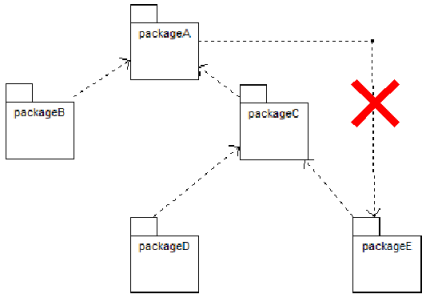
\includegraphics[width=9cm]{images/adp_1.png}
	}
	\begin{figure}[ht]
		\caption{\label{0}\textit{Gradle d�tectera un tel probl�me}}
	\end{figure}
\end{center}
%%%%%%%%%%%%%%%%%%%%%%%%%%%%%%%%%%%%%%%%%%%%%%%%%%%%%%%%%%%%%%%%%%%%%%%	

Dans chaque fichier {\tt build.gradle} on trouve les d�pendances du  module, par exemple dans le sous-projet {\tt navisu-intruments}  

\hbox{}\vspace{0.2cm}
{\small
	\begin{boxedverbatim}
		
dependencies {
    compile project(':navisu-core')
    compile project(':navisu-client')
    compile project(':navisu-domain')
    compile project(':navisu-app')
    compile project(':navisu-bathymetry')
    compile fileTree(dir: 'lib', include: '*.jar')
}

	\end{boxedverbatim}
}
\hbox{}\vspace{0.2cm}

Si le module {\tt navisu-app} devait instancier un {\tt Intrument} directement, il devrait connaitre, donc d�pendre du module {\tt navisu-intruments} ce qui constitue une rupture du principe num�ro deux.
Au lieu de cela les diff�rents {\tt Driver} s'inscrivent aupr�s de leur {\tt DriverManager} sp�cifique, 
ensuite lors d'une requ�te lanc�e par les callbacks du dock, le {\tt Driver} r�pondant aux crit�res de s�lection est activ�.

\hbox{}\vspace{0.2cm}
{\small
	\begin{boxedverbatim}
		
// class InstrumentDriverManagerImpl
	
protected List<InstrumentDriver> availableDriverList = new ArrayList<>();
	
@Override
public void registerNewDriver(InstrumentDriver driver) {
    Checker.notNull(driver, "Driver must not be null.");
    this.availableDriverList.add(driver);
}

@Override
public void open(String category) {
    InstrumentDriver driver = findDriver(category);
    if (driver != null) {
        driver.on();
    }else{
        System.out.println("Unrecognized instrument");
    }
}

protected InstrumentDriver findDriver(String category) {
    InstrumentDriver compatibleDriver = null;
    for (InstrumentDriver driver : this.availableDriverList) {
        if (driver.canOpen(category)) {
            compatibleDriver = driver;
            break;
        }
    }
    return compatibleDriver;
}
					
	\end{boxedverbatim}
}

\newpage
Exemple pour la classe {\tt Sonar} les m�thodes r�pondant au {\tt DriverManager}

\hbox{}\vspace{0.2cm}
{\small
	\begin{boxedverbatim}
		
// public class SonarImpl
              implements Sonar, SonarServices, InstrumentDriver, ComponentState {
              	
 private final String NAME = "Sonar";
 		
@Override
public boolean canOpen(String category) {
    return category.equals(NAME);
}
@Override
    public void on() {
        ...
}					
\end{boxedverbatim}
}
%%%%%%%%%%%%%%%%%%%%%%%%%%%%%%%%%%%%%%%%%%%%%%%%%%%%%%%%%%%%%%%%%%%%%%%
\chapter{Cartographie}
\section{Pr�sentation}

\nav\ utilise les cartes raster BSB/KAP. Avant d'utiliser vos cartes il est
n�cessaire d'op�rer un pr�-traitement, c'est l'op�ration de tuilage : la carte
au format KAP, de 1 � plusieurs Mo, sera transform�e en plusieurs sous images
ou tuiles. Les r�pertoires o� sont plac�s les cartes et les tuiles doivent �tre
renseign�s dans l'application.
\subsection{La projection Equirectangulaire}
%%%%%%%%%%%%%%%%%%%%%%%%%%%%%%%%%%%%%%%%%%%%%%%%%%%%%%%%%%%%%%%%%%%%%%
\nav, s'appuyant sur
\href{http://goworldwind.org/}{WorldWind},
utilise une projection cylindrique simple (appel�e projection
Equirectangulaire ou Plate Carr�e) avec comme r�f�rentiel g�od�sique le WGS84. Dans la projection Equirectangulaire
  l'instersection avec les m�ridiens se fait � angle droit, 
  mais contrairement � la projection Mercator, les parall�les sont des lignes
  droites �quidistantes.
%%%%%%%%%%%%%%%%%%%%%%%%%%%%%%%%%%%%%%%%%%%%%%%%%%%%%%%%%%%%%%%%%%%%%%%
\begin{center}
\framebox[1\width]{
	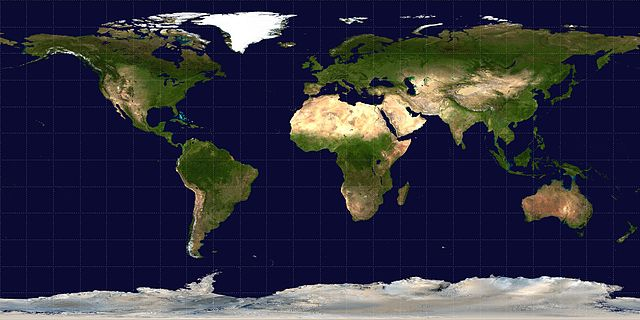
\includegraphics[width=16cm]{images/carto/Equirectangular-projection.png}
}
\begin{figure}[ht]
\caption{\label{equiProj}\textit{Projection �quirectangulaire}}
\end{figure}
\end{center}
%%%%%%%%%%%%%%%%%%%%%%%%%%%%%%%%%%%%%%%%%%%%%%%%%%%%%%%%%%%%%%%%%%%%%%%
Pour plus
d'informations sur le sujet consulter, par exemple,  le site du
``Intergovernmental Committee on Surveying and Mapping ``(ICSM) :
%%%%%%%%%%%%%%%%%%%%%%%%%%%%%%%%%%%%%%%%%%%%%%%%%%%%%%%%%%%%%%%%%%%%%%%

{
	\tt
	 \href{http://www.icsm.gov.au/mapping/about\_projections.html}{http://www.icsm.gov.au/mapping/about\_projections.html}
}\\

\vspace{.2cm}
%%%%%%%%%%%%%%%%%%%%%%%%%%%%%%%%%%%%%%%%%%%%%%%%%%%%%%%%%%%%%%%%%%%%%%%
Et pour un expos� plus large des probl�mes de projection :\\

\vspace{.2cm}
%%%%%%%%%%%%%%%%%%%%%%%%%%%%%%%%%%%%%%%%%%%%%%%%%%%%%%%%%%%%%%%%%%%%%%%
{
\tt 
	 \href{http://kartoweb.itc.nl/geometrics/}{http://kartoweb.itc.nl/geometrics/}
}
%%%%%%%%%%%%%%%%%%%%%%%%%%%%%%%%%%%%%%%%%%%%%%%%%%%%%%%%%%%%%%%%%%%%%%%

\subsection{Tuilage}
\subsubsection{Le principe}
Comme la plupart des applications g�or�f�renc�es (GoogleEarth, Yahoo, Bing,
\ldots) pour fournir un niveau de d�tail important et une bonne fluidit�,
\nav\ utilise la m�thode du tuilage des cartes. Les images affich�es sont de
256x256 pixels. Elles sont choisies suivant le niveau de zoom et l'emplacement
g�ographique, l'affichage � l'�cran est recr�� dynamiquement.
Chaque carte est constitu�e d'un r�pertoire, puis de nombreux sous-r�pertoires
num�rot�s comme suit :
%%%%%%%%%%%%%%%%%%%%%%%%%%%%%%%%%%%%%%%%%%%%%%%%%%%%%%%%%%%%%%%%%%%%%%%
\begin{center}
\framebox[1\width]{
	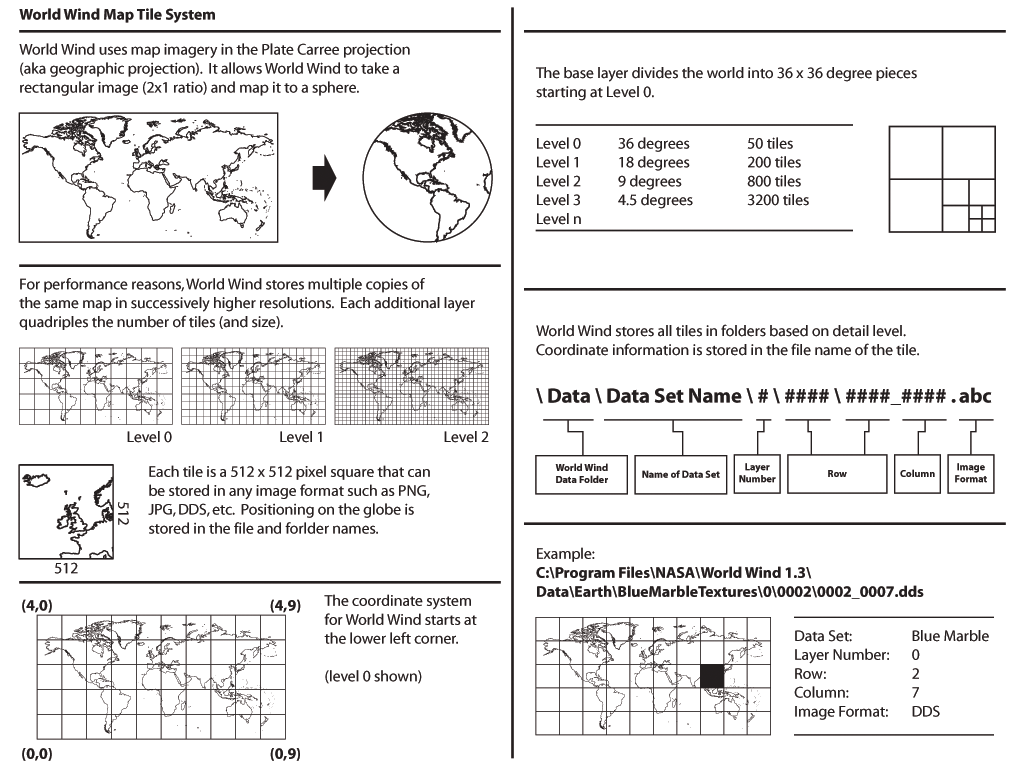
\includegraphics[width=16cm]{images/carto/Worldwind_tile_system.png}
}
\begin{figure}[ht]
\caption{\label{wwTiles}\textit{Conventions de la num�rotation des
tuiles WorldWind}}
\end{figure}
\end{center}
 Lors d'un
premier acc�s ces images peuvent provenir de diff�rents sites internet, elles
sont mises en cache sur le disque utilisateur. Lors des acc�s suivants
l'application commence par chercher dans le cache. Elles peuvent �tre d�s le
d�part �tre mise dans le cache.\\
 Sous Windows 7 par d�faut WorldWind utilise le
r�pertoire :
\begin{verbatim} C:\ProgramData\WorldWindData \end{verbatim} 

Pour plus de d�tails sur le tuilage, voir :

%%%%%%%%%%%%%%%%%%%%%%%%%%%%%%%%%%%%%%%%%%%%%%%%%%%%%%%%%%%%%%%%%%%%%%%
\begin{center}
	 \href{http://www.worldwindcentral.com/wiki/Tiling\_System}{http://www.worldwindcentral.com/wiki/Tiling\_System}
\end{center}
%%%%%%%%%%%%%%%%%%%%%%%%%%%%%%%%%%%%%%%%%%%%%%%%%%%%%%%%%%%%%%%%%%%%%%%
\section{Cartographie raster}
\subsection{Les cartes BSB/KAP}
 L'utilisateur peut d�finir son
propre r�pertoire pour passer facilement d'un ordinateur � un autre, sans avoir � recopier les donn�es.


%%%%%%%%%%%%%%%%%%%%%%%%%%%%%%%%%%%%%%%%%%%%%%%%%%%%%%%%%%%%%%%%%%%%%%%
\begin{center}
\framebox[1\width]{
	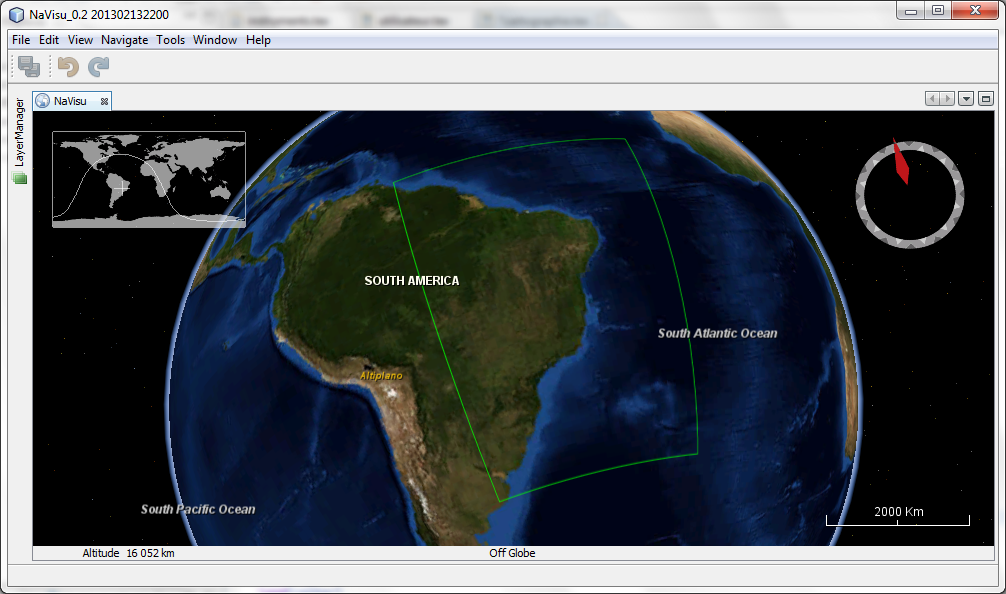
\includegraphics[width=16cm]{images/carto/0.png}
}
\begin{figure}[ht]
\caption{\label{carte0}\textit{Fronti�res d'une carte}}
\end{figure}
\end{center}
%%%%%%%%%%%%%%%%%%%%%%%%%%%%%%%%%%%%%%%%%%%%%%%%%%%%%%%%%%%%%%%%%%%%%%%
Les fronti�res sont en vert : la carte 101.KAP est dans le r�pertoire d�sign� et
la carte a �t� tuil�e, les tuiles sont dans le cache d�sign�. Si les tuiles ne
sont pas dans le cache les polygones fronti�re sont rouges.
%%%%%%%%%%%%%%%%%%%%%%%%%%%%%%%%%%%%%%%%%%%%%%%%%%%%%%%%%%%%%%%%%%%%%%%
\begin{center}
\framebox[1\width]{
	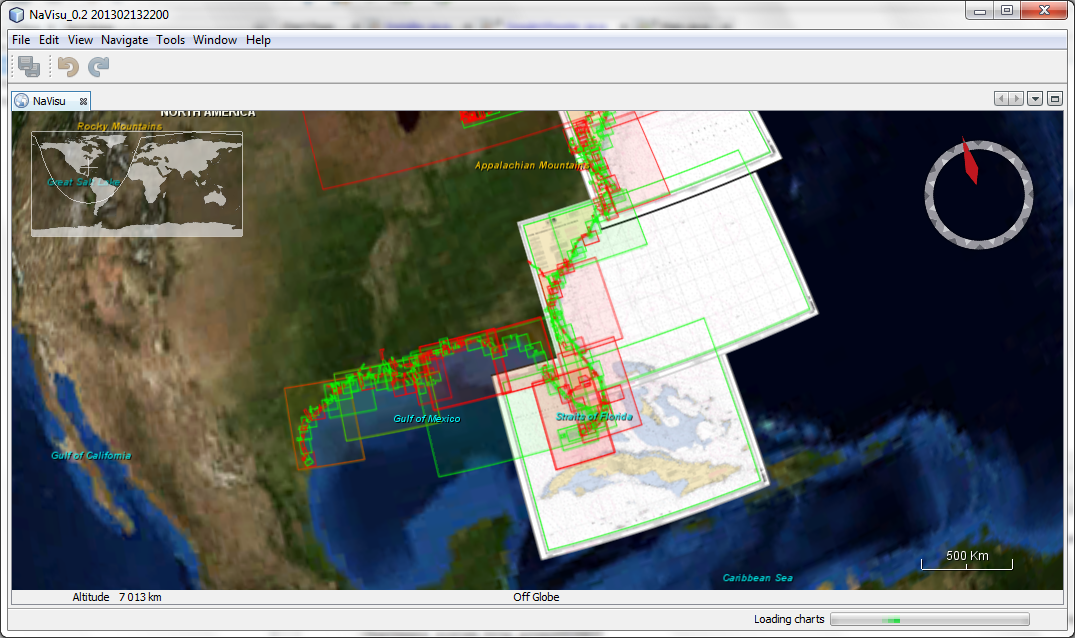
\includegraphics[width=16cm]{images/carto/3.png}
}
\begin{figure}[ht]
\caption{\label{usa}\textit{Les Etats Unis}}
\end{figure}
\end{center}
%%%%%%%%%%%%%%%%%%%%%%%%%%%%%%%%%%%%%%%%%%%%%%%%%%%%%%%%%%%%%%%%%%%%%%%
%%%%%%%%%%%%%%%%%%%%%%%%%%%%%%%%%%%%%%%%%%%%%%%%%%%%%%%%%%%%%%%%%%%%%%%
\begin{center}
\framebox[1\width]{
	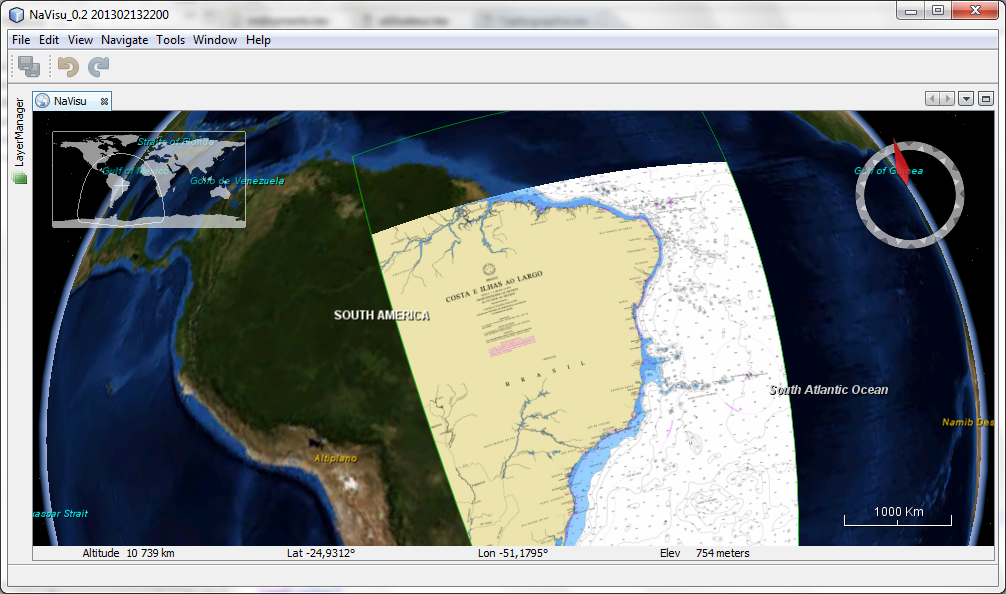
\includegraphics[width=16cm]{images/carto/1.png}
}
\begin{figure}[ht]
\caption{\label{carte1}\textit{Affichage de la carte}}
\end{figure}
\end{center}
%%%%%%%%%%%%%%%%%%%%%%%%%%%%%%%%%%%%%%%%%%%%%%%%%%%%%%%%%%%%%%%%%%%%%%%
Double clic � l'int�rieur du polygone : affichage de la carte, d�s que
l'altitude le permet.
Ici la distance fait que les tuiles les plus hautes en latitude ne s'affichent pas encore.
%%%%%%%%%%%%%%%%%%%%%%%%%%%%%%%%%%%%%%%%%%%%%%%%%%%%%%%%%%%%%%%%%%%%%%%
\begin{center}
\framebox[1\width]{
	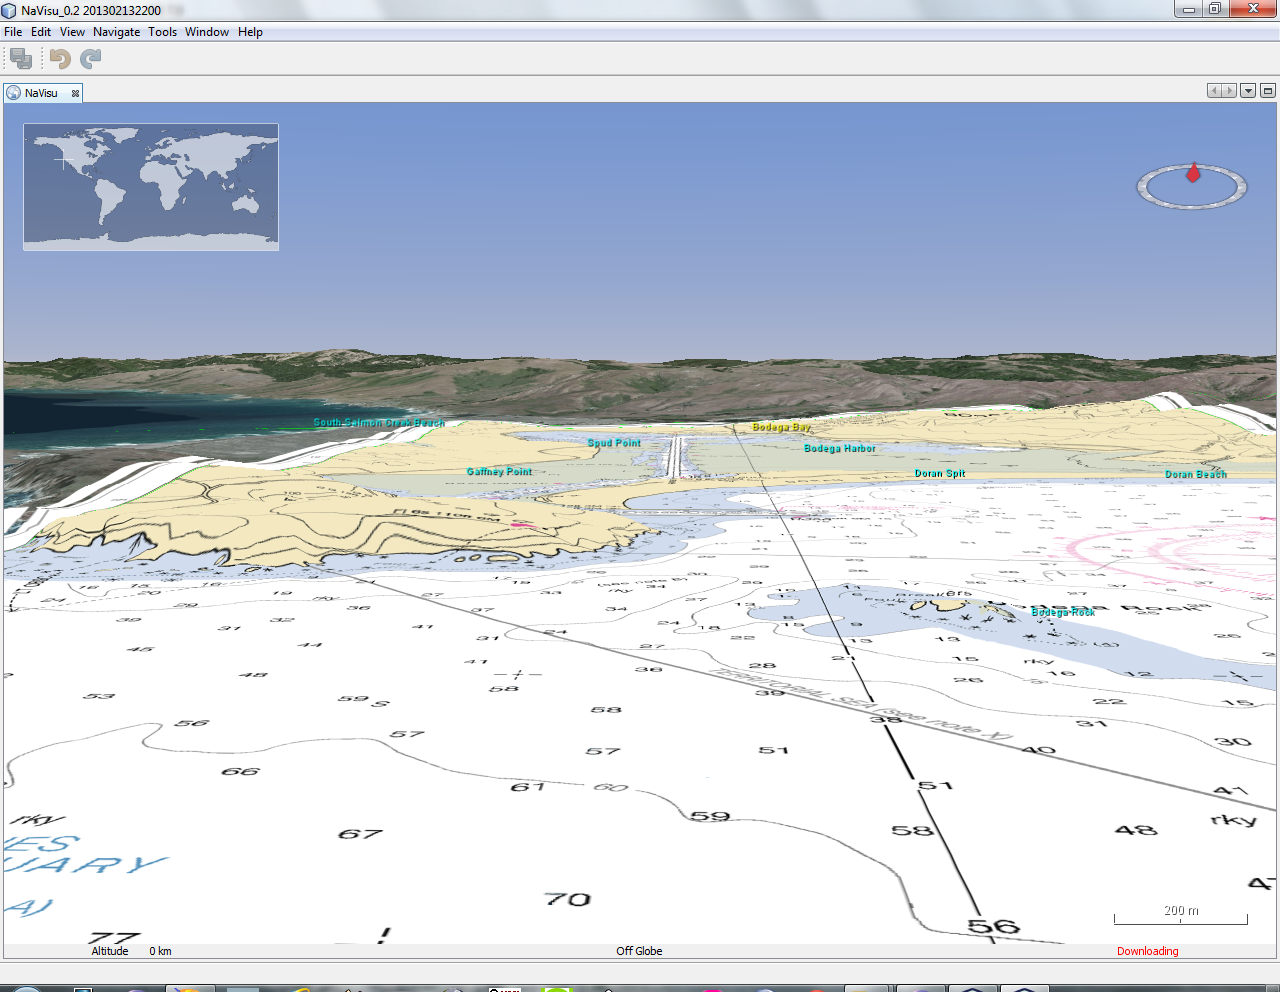
\includegraphics[width=16cm]{images/carto/2.png}
}
\begin{figure}[ht]
\caption{\label{details}\textit{Niveaux de d�tail et la 3D}}
\end{figure}
\end{center}
%%%%%%%%%%%%%%%%%%%%%%%%%%%%%%%%%%%%%%%%%%%%%%%%%%%%%%%%%%%%%%%%%%%%%%%
\subsection{Acquisition}
Quelques sites pour obtenir des cartes raster au format BSB/KAP : 
%%%%%%%%%%%%%%%%%%%%%%%%%%%%%%%%%%%%%%%%%%%%%%%%%%%%%%%%%%%%%%%%%%%%%%%

{
\tt\small
	 \href{http://marine.geogarage.com/}{http://marine.geogarage.com/}
	 
	 \vspace{.2cm}
	\href{http://www.justmagic.com/RasterChart2BSB.html}{http://www.justmagic.com/RasterChart2BSB.html}
	
	\vspace{.2cm}
	 \href{https://www.mar.mil.br/dhn/chm/cartas/download/cartasbsb/cartas\_eletronicas\_Internet.htm}{https://www.mar.mil.br/dhn/chm/cartas/download/cartasbsb/cartas\_eletronicas\_Internet.htm}
	
	\vspace{.2cm}
	 \href{http://www.nauticalcharts.noaa.gov/mcd/Raster/index.htm}{http://www.nauticalcharts.noaa.gov/mcd/Raster/index.htm}
	
	 \vspace{.2cm}
	 \href{http://www.1yachtua.com/}{http://www.1yachtua.com/}
	 
}
%%%%%%%%%%%%%%%%%%%%%%%%%%%%%%%%%%%%%%%%%%%%%%%%%%%%%%%%%%%%%%%%%%%%%%%



	\newpage
	\label{fin}
	
	% ------------------------------------------------------------------------------
\end{document}
